% Options for packages loaded elsewhere
\PassOptionsToPackage{unicode}{hyperref}
\PassOptionsToPackage{hyphens}{url}
%
\documentclass[
]{article}
\usepackage{lmodern}
\usepackage{amsmath}
\usepackage{ifxetex,ifluatex}
\ifnum 0\ifxetex 1\fi\ifluatex 1\fi=0 % if pdftex
  \usepackage[T1]{fontenc}
  \usepackage[utf8]{inputenc}
  \usepackage{textcomp} % provide euro and other symbols
  \usepackage{amssymb}
\else % if luatex or xetex
  \usepackage{unicode-math}
  \defaultfontfeatures{Scale=MatchLowercase}
  \defaultfontfeatures[\rmfamily]{Ligatures=TeX,Scale=1}
\fi
% Use upquote if available, for straight quotes in verbatim environments
\IfFileExists{upquote.sty}{\usepackage{upquote}}{}
\IfFileExists{microtype.sty}{% use microtype if available
  \usepackage[]{microtype}
  \UseMicrotypeSet[protrusion]{basicmath} % disable protrusion for tt fonts
}{}
\makeatletter
\@ifundefined{KOMAClassName}{% if non-KOMA class
  \IfFileExists{parskip.sty}{%
    \usepackage{parskip}
  }{% else
    \setlength{\parindent}{0pt}
    \setlength{\parskip}{6pt plus 2pt minus 1pt}}
}{% if KOMA class
  \KOMAoptions{parskip=half}}
\makeatother
\usepackage{xcolor}
\IfFileExists{xurl.sty}{\usepackage{xurl}}{} % add URL line breaks if available
\IfFileExists{bookmark.sty}{\usepackage{bookmark}}{\usepackage{hyperref}}
\hypersetup{
  pdftitle={Visualize 120 Years of Summer Olympics},
  pdfauthor={Chris Fang \& Hongtao Hao},
  hidelinks,
  pdfcreator={LaTeX via pandoc}}
\urlstyle{same} % disable monospaced font for URLs
\usepackage{longtable,booktabs}
\usepackage{calc} % for calculating minipage widths
% Correct order of tables after \paragraph or \subparagraph
\usepackage{etoolbox}
\makeatletter
\patchcmd\longtable{\par}{\if@noskipsec\mbox{}\fi\par}{}{}
\makeatother
% Allow footnotes in longtable head/foot
\IfFileExists{footnotehyper.sty}{\usepackage{footnotehyper}}{\usepackage{footnote}}
\makesavenoteenv{longtable}
\usepackage{graphicx}
\makeatletter
\def\maxwidth{\ifdim\Gin@nat@width>\linewidth\linewidth\else\Gin@nat@width\fi}
\def\maxheight{\ifdim\Gin@nat@height>\textheight\textheight\else\Gin@nat@height\fi}
\makeatother
% Scale images if necessary, so that they will not overflow the page
% margins by default, and it is still possible to overwrite the defaults
% using explicit options in \includegraphics[width, height, ...]{}
\setkeys{Gin}{width=\maxwidth,height=\maxheight,keepaspectratio}
% Set default figure placement to htbp
\makeatletter
\def\fps@figure{htbp}
\makeatother
\setlength{\emergencystretch}{3em} % prevent overfull lines
\providecommand{\tightlist}{%
  \setlength{\itemsep}{0pt}\setlength{\parskip}{0pt}}
\setcounter{secnumdepth}{5}
\usepackage{booktabs}

% \usepackage{makeidx}
% \makeindex

\urlstyle{tt}

\usepackage{amsthm}
\makeatletter
\def\thm@space@setup{%
  \thm@preskip=8pt plus 2pt minus 4pt
  \thm@postskip=\thm@preskip
}
\makeatother
\ifluatex
  \usepackage{selnolig}  % disable illegal ligatures
\fi
\usepackage[]{natbib}
\bibliographystyle{plainnat}

\title{Visualize 120 Years of Summer Olympics}
\author{Chris Fang \& Hongtao Hao}
\date{2021-01-23}

\begin{document}
\maketitle

{
\setcounter{tocdepth}{2}
\tableofcontents
}
\hypertarget{preface}{%
\section*{Preface}\label{preface}}
\addcontentsline{toc}{section}{Preface}

This data visualization project was completed by Zihui (Chris) Fang and Hongtao Hao, with Equal Contribution, as the term paper for Professor Yong-Yeol Ahn's Data Visualization course in 2019 Fall.

This study analyzed the historical data which contains information on athletes in all the past modern Olympic Games. We tried to answer four questions:

\begin{enumerate}
\def\labelenumi{\arabic{enumi}.}
\item
  How did female participation change over the years and how did these changes differ between continents?
\item
  Is there a home-field advantage at the Olympics?
\item
  How ``efficient'' is each participating country or region to get medals? and
\item
  Which sports had the highest number of participants?
\end{enumerate}

Results showed that both total number of athletes and the rate of female participation have been increasing in the past 120 years. Also, there seems to exist a home-field advantage. Third, medal efficiency is highly correlated with participating country or region's economic development. Finally, athletics, gymnastics, and swimming have the highest number of athletes.

You can also download the \href{https://raw.githubusercontent.com/hongtaoh/olymvis/master/static/tex-pdf/fang_hao_olymvis.pdf}{PDF version} of our paper, whose LaTex source code can be found \href{https://github.com/hongtaoh/olymvis/blob/master/static/tex-pdf/fang_hao_olymvis.tex}{here}.

\hypertarget{abstract}{%
\section*{Abstract}\label{abstract}}
\addcontentsline{toc}{section}{Abstract}

From the first modern Olympics in 1896 to Rio 2016, the Summer Olympic Games has been through 120 years. This study analyzed the \href{https://github.com/rgriff23/Olympic_history}{historical data} about the Olympics and tried to answer four questions, i.e.,

\begin{itemize}
\item
  how female participation changed over the years and how these changes differed between continents,
\item
  whether there is a home-field advantage at the Olympics,
\item
  how ``efficient'' is each participating country and region to get medals, and
\item
  which sports had the highest number of participants.
\end{itemize}

Results showed that both total number of athletes and the rate of female participation have been increasing in the past 120 years. Also, there seems to exist a home-field advantage. Third, medal efficiency is highly correlated with participating country or region's economic development. Finally, athletics, gymnastics, and swimming have the highest number of athletes.

\hypertarget{motivation}{%
\section{Motivation}\label{motivation}}

The modern Olympic Games are the greatest sports mega-event in the world (Grix, 2013). It generates a massive number of audiences worldwide. The latest Rio 2016 Olympics, for example, attracted 3.5 billion viewers (Roxbourough, 2016), half of the world population. Apart from this mobilizing power, the Olympic Games have significant political (Giulianotii, 2015; Cottrell \& Nelson, 2010; MacAloon, 1995), economic (Madden, 2002; Blake, 2005; Osada, Ojima, Kurachi, Miura, \& Kawamoto, 2016), and socio-cultural (Malfas, Theodoraki, \& Houlihan, 2004) impacts. It also contributes to global friendship and cooperation (Beutler, 2008).

Gender equality in sports has been a hot topic (Mervosh \& Caron, 2019). Debates on this issue have revolved around equal pay and media coverage (Baker, Seymour, \& Zimbalist, 2019). There has long been an obvious gender pay gap in sports (Abrams, 2019; Farmer, 2017). For example, of the 100 athletes on the 2019 Forbes list of the world's highest-paid athletes, only one of them is a woman. i.e., Serena Williams, who is ranked 63th on the list. There has also been a lack of media coverage on women in sports. Although 40\% of all sports participants are female, only 4\% of the sports media coverage were about female athletes (MacKenzie, 2019). A study (Cooky, Messner, \& Musto, 2015) examining sports coverage from 1989 to 2014 found that despite a dramatic increase in the number of women playing sports (Good, 2015), there had been a decrease in the amount of coverage of female athletes. Under this backdrop, we aim to look at female participation across the globe in the Summer Olympic Games of the past 120 years.

Recently, there has been a trend that fewer cities want to host the Olympics, challenging the future of a century-old tradition (Goldblatt, 2016). For example, 12 cities bid for 2004 Summer Olympics but only two for the 2020 Winter games (Ludacer, 2018). Considering the importance of Olympic success in national pride (Mower, 2012), a home-field advantage in the Olympics might encourage countries to bid for hosting the mega-event. Therefore, it is worth investigating whether this advantage exists in the Olympics, and how significant it is.

Although earning medals can boost national pride, countries are not ``born equal'' in terms of their ability to achieve Olympic success. Studies have demonstrated that population sizes and economic development for a large part determined a country's Olympic performance (Soos, Martinez, \& Szabo, 2017; Xun, 2005; Bernard \& Busse, 2004). However, we think it's unfair to compare Singapore with the United States in terms of total number of medals earned, because the two countries have totally different population size. What is more important is ``medal efficiency'', i.e., medal counts per athlete participating in the Olympics. In other words, we are more concerned about how effective a country is to earn medals, rather than the total number of medals earned. We aim to look at how this ``medal efficiency'' differs between countries.

Apart from its significance for societies at large, Olympics is associated with individuals' health as well (Sandercocok, Beedie, \& Mann, 2016). People might be inspired by the Olympics and more actively engage in physical activities. Besides its benefits for physical health (Warburton, Nicol, \& Bredin, 2006), it has psychological benefits as well (Ghildiyal, 2015). For example, playing sports can help build one's characters. With the importance of sports in mind, we want to examine which sports in the Olympics history have the highest number of participants.

\hypertarget{lit}{%
\section{Litrature Review}\label{lit}}

In the following, we'll review relevant literature.

\hypertarget{lit-female}{%
\subsection{Female Participation in Summer Olympics}\label{lit-female}}

Many attempts have already been made to visualize female participation in the Olympics. The most basic one (Bmallion, 2015) is using tables to display the information about countries with the highest and lowest percentages of female athletes, and to show female percentages across the 120 years of the Olympics. See Table 1.

\begin{figure}
\centering
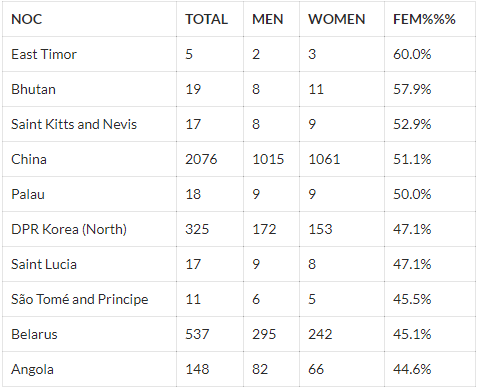
\includegraphics[width=0.5\textwidth,height=\textheight]{static/pics/1-1.png}
\caption{Table 1(a): Countries with the highest rate of female participation}
\end{figure}

\begin{figure}
\centering
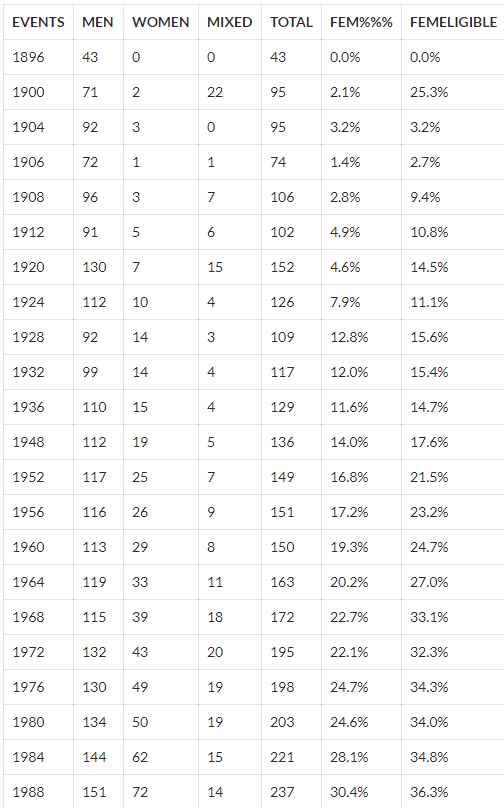
\includegraphics[width=0.5\textwidth,height=\textheight]{static/pics/1-2.png}
\caption{Table 1(b): Female percentage in Olympic events}
\end{figure}

This method is simple and informative. This is useful for researchers looking for information on this topic, but it is not effective in terms of visualization. For example, looking at the plain number won't help viewers have a clear idea of the trend in female participation in the past 120 years.

Another simple but effective method is using a line graph displaying the number of female and male athletes in each Olympic Games from 1896 to 2016 (Nunes, 2019). See Figure \ref{fig:figure01}.

\begin{figure}

{\centering 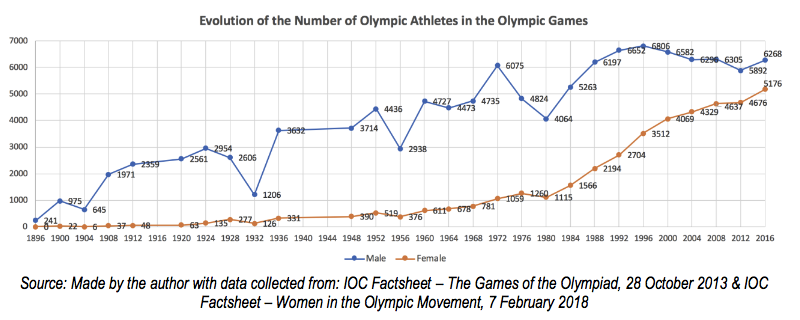
\includegraphics[width=1\linewidth]{static/pics/1-3} 

}

\caption{Evolution of the number of Olympic athletes, male and female (1986-2016), Nunes (2019)}\label{fig:figure01}
\end{figure}

This graph is successful in showing the growth in the number of female athletes. However, it fails to show the percentage change. Although viewers can see directly the increase in the total number, they might find it difficult to notice the changes in the percentage.

\emph{Washington Street Journal} did an interactive visualization comparing the inclusion of female and male events in the Olympics history (Serkez, 2018). It clearly shows that most men's events were already established before the 1960s, whereas most women's events were only introduced after the 1980s. See Figure \ref{fig:figure02}.

\begin{figure}

{\centering 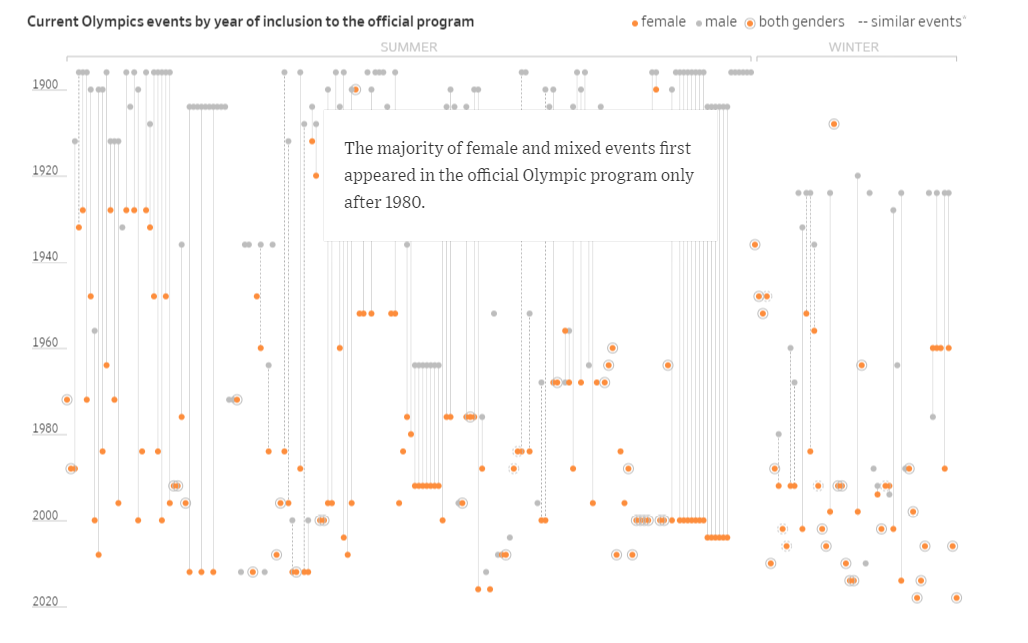
\includegraphics[width=0.95\linewidth]{static/pics/1-4} 

}

\caption{Interactive plot by Washington Post showing inclusion of male and female Olympic events}\label{fig:figure02}
\end{figure}

Each individual dot represents a sport of a gender. When clicked, there will be a line connecting to the same sport of a different gender, and information on the inclusion of this sport for both genders will appear. Overall, this visualization clearly shows how late the introduction of female events was in the Olympics history, but it did not show how the number and percentage of female athletes changed over the years.

The official website of the International Olympic Committee (IOC) also made an attempt to show the growth in the percentage of sportswomen in the Olympics. See Figure \ref{fig:figure03}.

\begin{figure}

{\centering 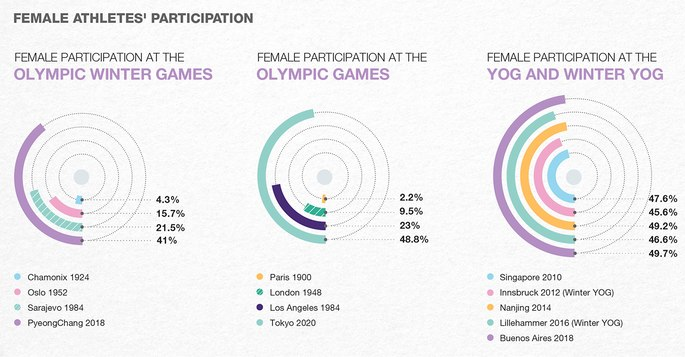
\includegraphics[width=0.95\linewidth]{static/pics/1-5} 

}

\caption{IOC graph visualizing female athletes' participation}\label{fig:figure03}
\end{figure}

As can be seen, it is effective in the way that it shows the dramatic changes in female participation by showing four Olympics in each of the charts. However, its drawback is obvious: the number of Olympic Games that are able to be displayed is extremely limited. It is impossible to show the information of all the Olympics in the past 120 years using this method.

Although there were many attempts visualizing the evolution of female participation in general, few visualizations exist showing the percentage change by continent. The only piece we found is several tables showing men and women participation in the Olympics from 1996 to 2016. No visualizations on this information were made. We decided that there is a gap here. Although both the total number and relative percentage of female athletes have been growing (Nunes, 2019), the increase might be different between continents. We decided to take a closer look at this in our study.

\hypertarget{lit-homefield}{%
\subsection{Home-field Advantage}\label{lit-homefield}}

Similar to the attempt at showing female participation, simple and basic tables were utilized to examine the existence of home-field advantage at the Olympics (Pettigrew \& Reiche, 2016). See Figure \ref{fig:figure04}.

\begin{figure}

{\centering 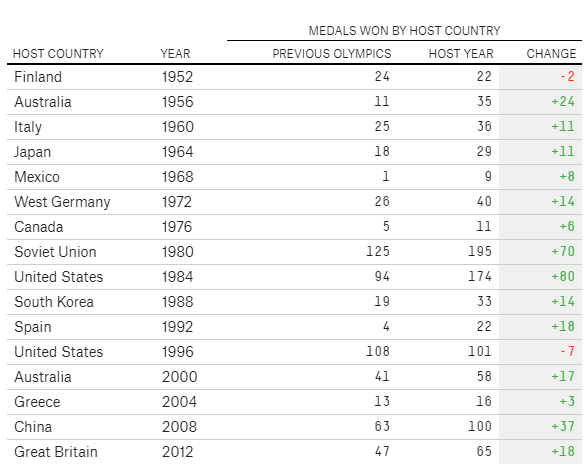
\includegraphics[width=0.85\linewidth]{static/pics/2-1} 

}

\caption{Medals won by host countries at host year and the previous Olympics, Pettigrew and Reiche (2016)}\label{fig:figure04}
\end{figure}

This visualization shows a table comparing the total number of medals earned at the host year and the previous Olympics. Changes between the two were shown in the last column. Among the 16 host countries from 1952 to 2012, only two countries showed negative changes, meaning that hosting the Olympics helped the country earn more medals. However, the problem with this method is that it is a little bit arbitrary to compare the host year and the adjacently previous Olympics. Changes might have been positive simply because these countries did not perform well only in the previous Games, even though they had performed well eight or more years before the host year. Therefore, it is a more robust choice to show these countries' Olympic performances in all years.

Clarke (2000) did this by calculating the ``Home: Away Ratio''. See Table 2.

\begin{figure}
\centering
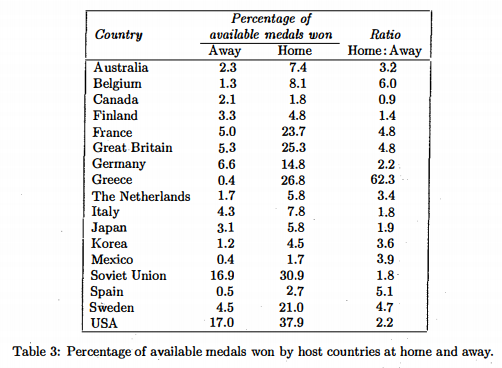
\includegraphics[width=0.8\textwidth,height=\textheight]{static/pics/2-3.png}
\caption{Table 2: Percentage of available medals won by host countries at home and away, Clarke (2016)}
\end{figure}

He listed the percentage of all available medals won by countries that have ever hosted an Olympic both at the Home years and the Away years. The ratio of ``Home: Away'' was calculated. Obviously, a ratio larger than 1 indicates the existence of home-field advantage at the Olympics. The drawback of this method is that it only shows the summary of all the years, lacking information about these countries' performance in each year.

Visualizations showing all the years do exist (Grange, 2016). See Figure \ref{fig:figure05}.

\begin{figure}

{\centering 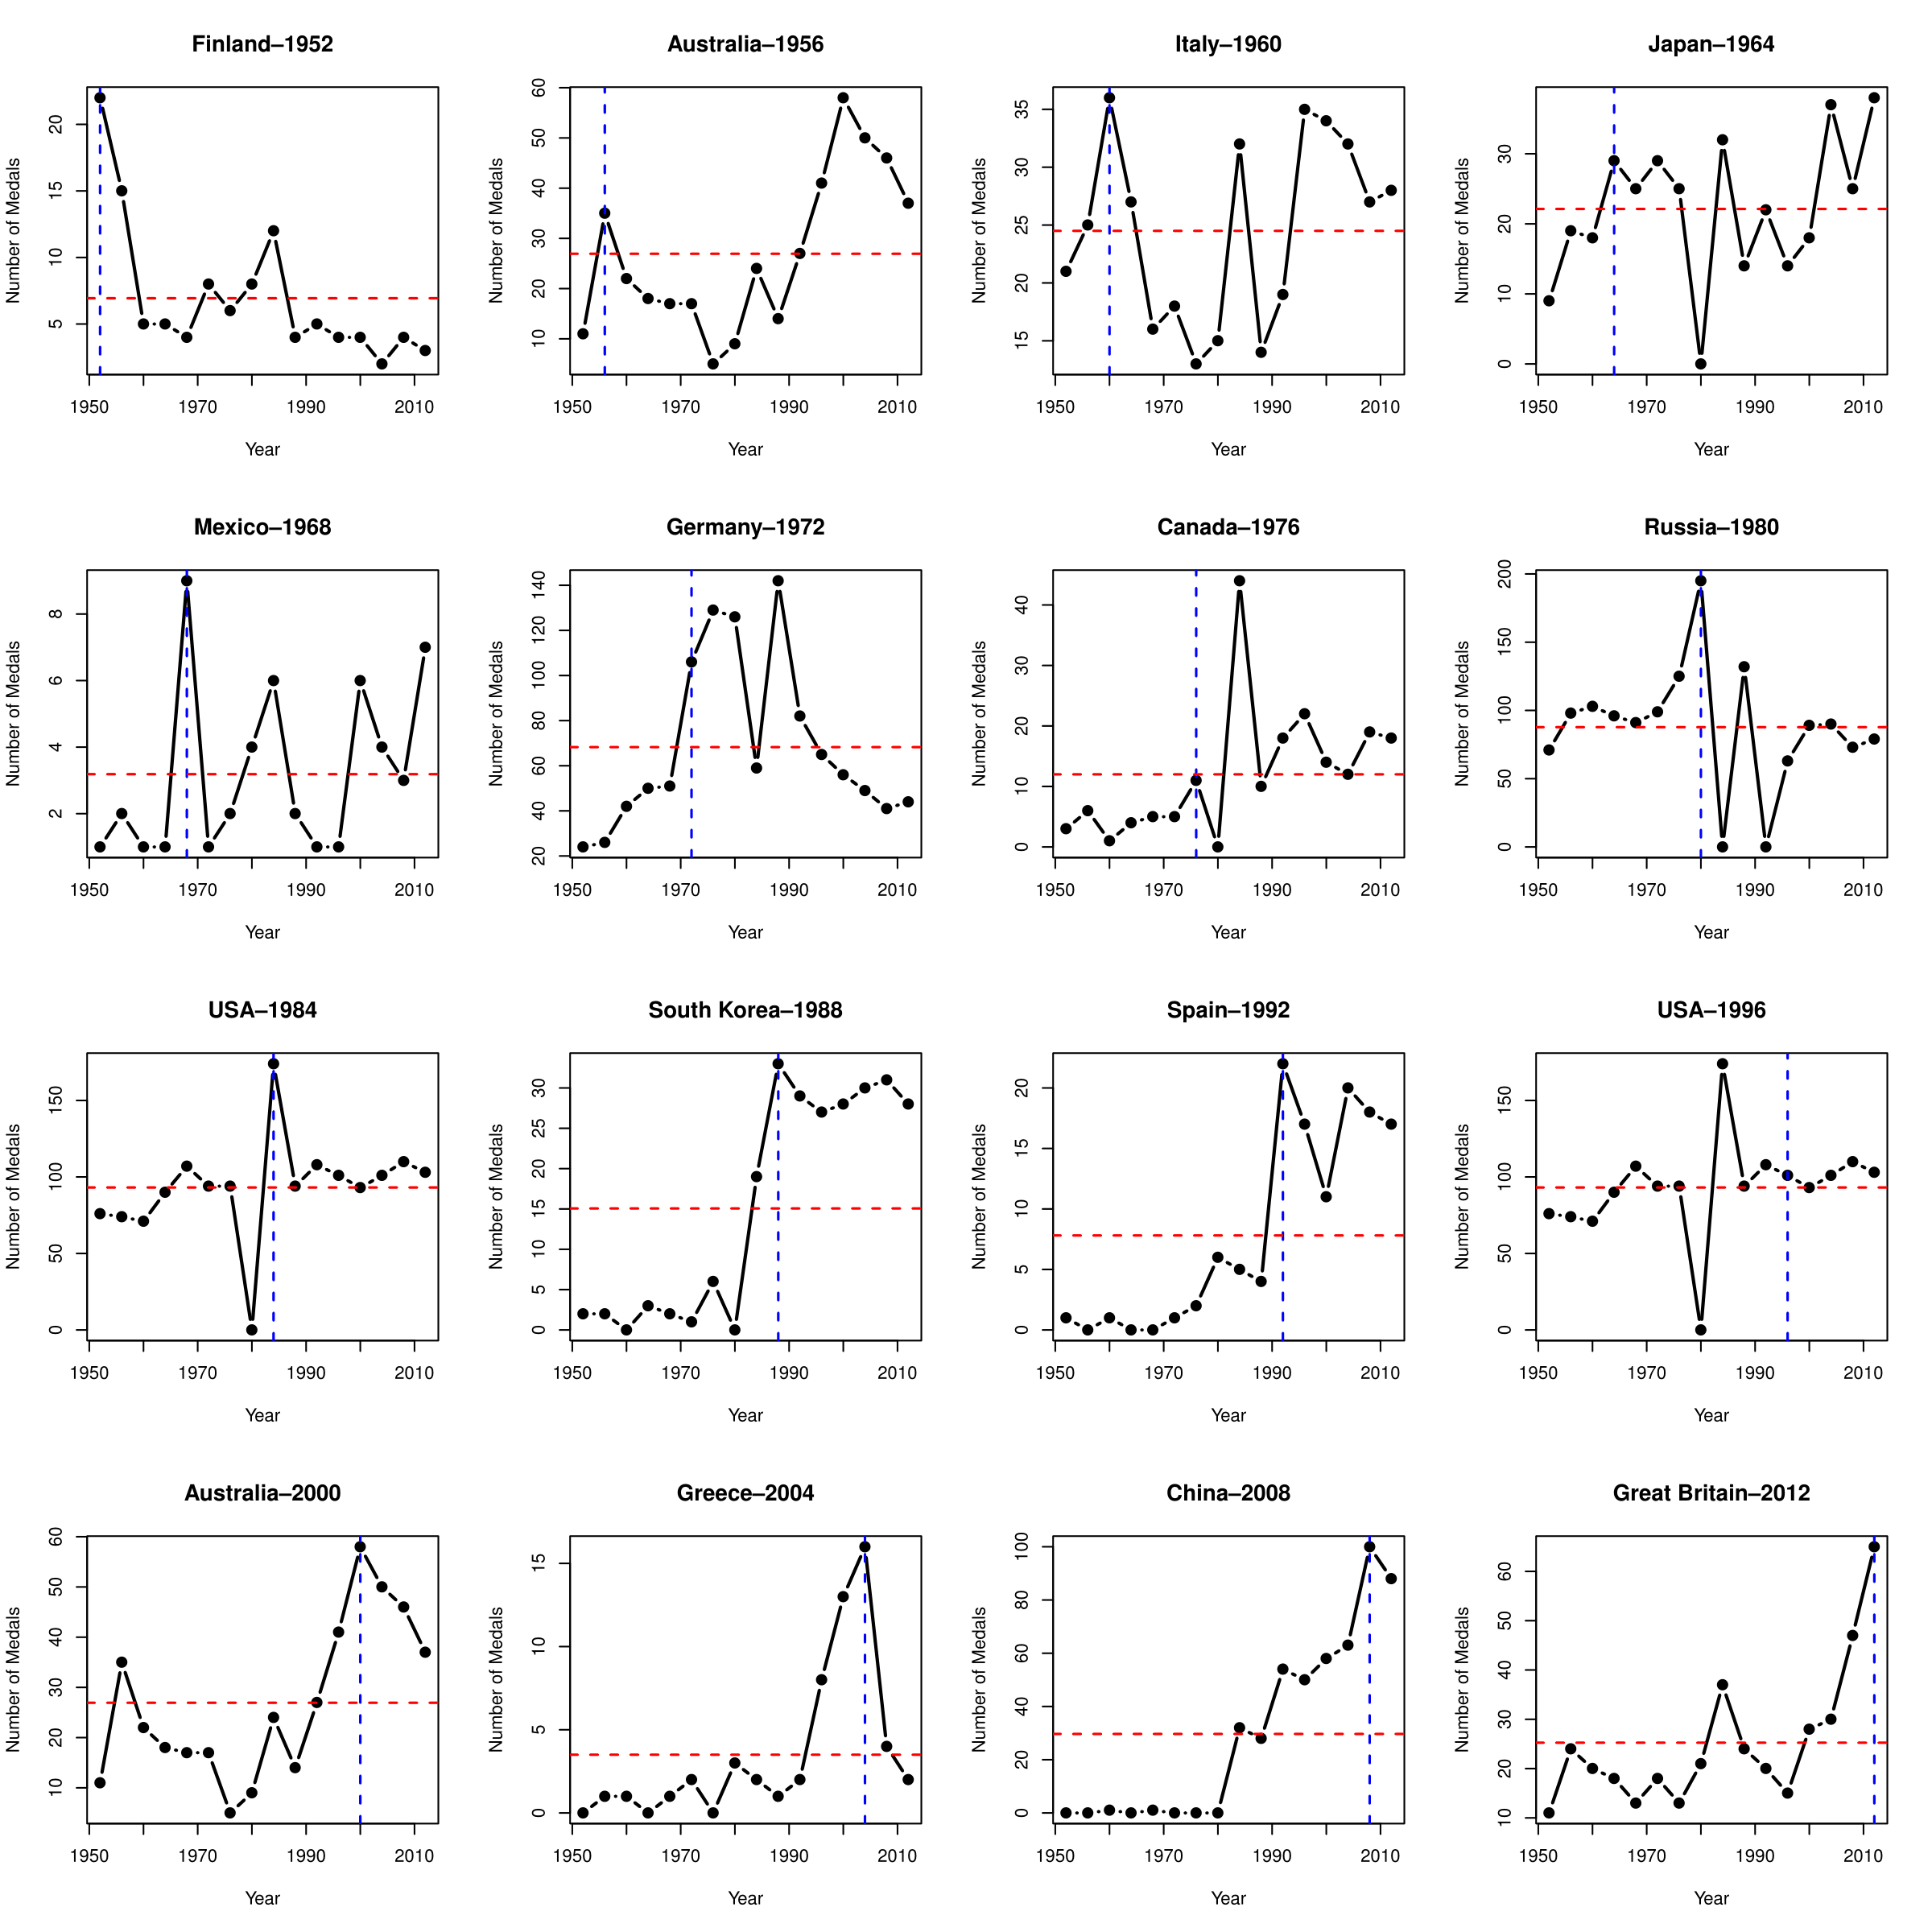
\includegraphics[width=1.2\linewidth]{static/pics/2-2} 

}

\caption{Visualizing home-field advantage by Grange (2006)}\label{fig:figure05}
\end{figure}

For example, in this small multiple made by R, each graph has a blue vertical line emphasizing the number of medals earned during the host year, and a red horizontal line indicating the total average. It is very effective in the sense that it clearly compares the performance during the host year and all other years. The problem with this method is that lines are not very good at showing density distribution of medal numbers over the years. To improve this drawback, we decided to use kernel density estimation (KDE) coupled with small multiples.

\hypertarget{lit-medal}{%
\subsection{Medal Efficiency}\label{lit-medal}}

The most straightforward way of measuring a country's efficiency of earning medals is to count the number of medals per athlete participating. This method was used by Pettigrew and Reiche (2016) in their analysis of home-field advantage.

Some scholars argued that when assessing the efficiency of medal production, we need to take into account the resources that countries possess, such as GDP and population. From an economics perspective, Rathke and Woitek (2007) came up with a sophisticated formula calculating this efficiency, and visualized the results using multiple box plots that were stacked horizontally. See Figure \ref{fig:figure06}.

\begin{figure}

{\centering 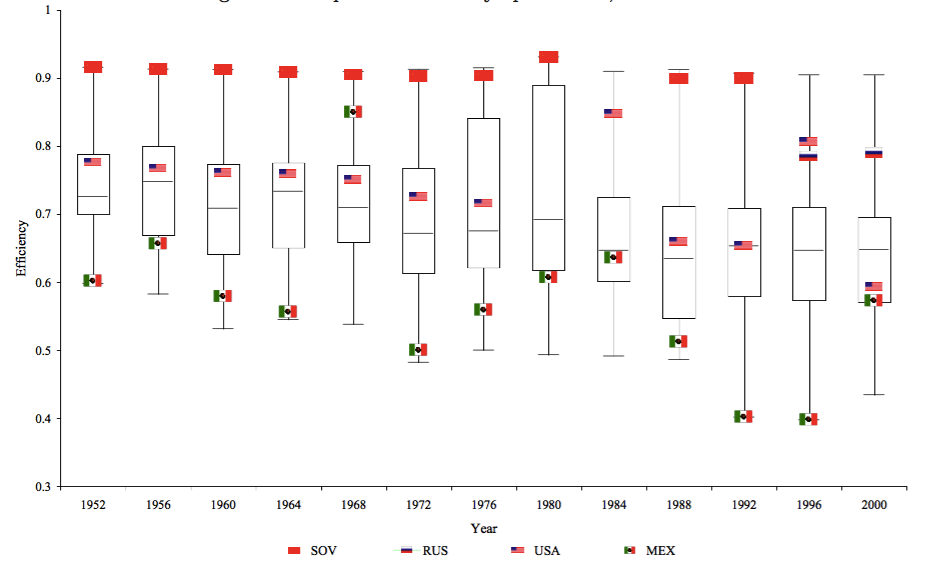
\includegraphics[width=0.95\linewidth]{static/pics/3-2} 

}

\caption{The production of Olympic Medals, 1952-2000, Rathke and Wotiek (2007)}\label{fig:figure06}
\end{figure}

Visualizations by Eirk (2016) for the \emph{Telegraph}, and those by medalspercapita.com also highlighted the importance of GDP and the size of population. For example, Eirk (2016) ranked Olympic nations based on ``Gold per million people'' and ``Gold per £100 bn GDP''. See Figure \ref{fig:figure07} and \ref{fig:figure08}.

\begin{figure}

{\centering 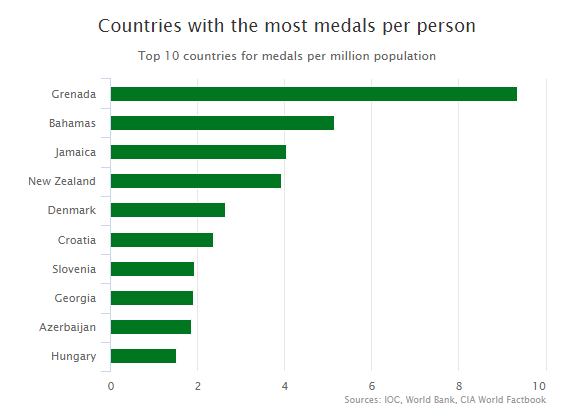
\includegraphics[width=0.9\linewidth]{static/pics/3-3} 

}

\caption{Top 10 countries for medals per million population, Eirk (2006)}\label{fig:figure07}
\end{figure}

\begin{figure}

{\centering 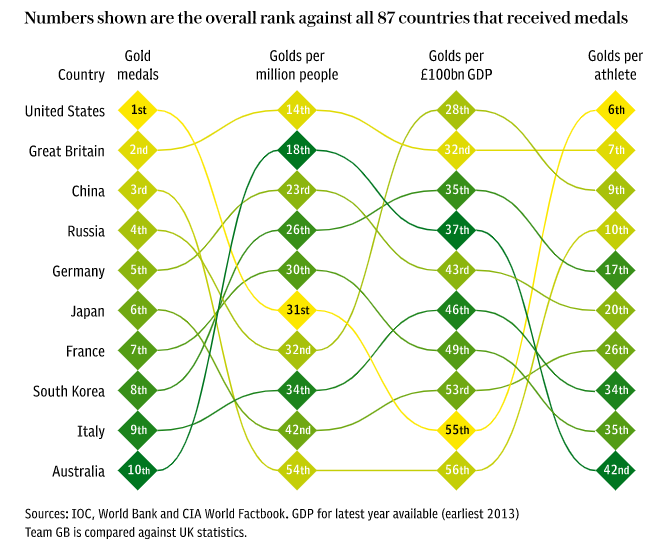
\includegraphics[width=0.85\linewidth]{static/pics/3-4} 

}

\caption{Ranking medal production considering population and GDP, Eirk (2006)}\label{fig:figure08}
\end{figure}

Similarly, using the concept of ``medals per capita'', medalspercapita.com ranked countries based on ``population per medal'', i.e., how many people are needed to generate a medal. They created a choropleth map based on the results where darker colors indicate lower ``medals per capita''. See Table 3 and Figure \ref{fig:figure09}.

\begin{figure}
\centering
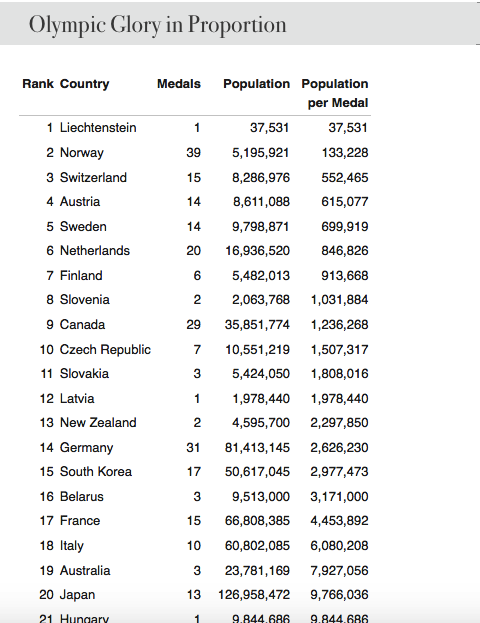
\includegraphics[width=0.7\textwidth,height=\textheight]{static/pics/3-5.png}
\caption{Table 3: Population per medal}
\end{figure}

\begin{figure}

{\centering 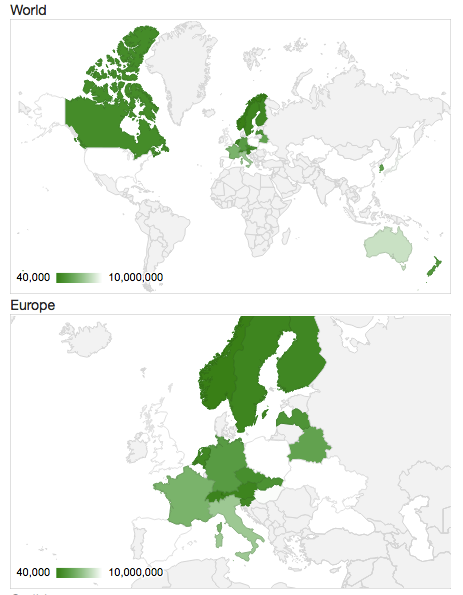
\includegraphics[width=0.7\linewidth]{static/pics/3-6} 

}

\caption{World map of population per medal}\label{fig:figure09}
\end{figure}

However, we think it is problematic to divide medal counts by population or GDP in measuring medal efficiency. First of all, this method is unfair for countries who joined the Olympics late. For example, China (PRC) attended the Olympics for the first time in 1952 and due to political issues, it was not a participant till 1984 (COC, 2004). If the total number of medals is the basis for medal efficiency, it would be unfair for countries like China and many newly founded countries in Africa.

Second, it might be unfair to divide the number of medals by population. This formula assumes that a country can send as many athletes as it wants, but this is not the case. For example, for Tokyo 2020, each country can send at most three male and three female athletes (International Table Tennis Federation, 2018). As a result, China will send six table tennis athletes, as will Australia, Japan, Brazil, Egypt, Germany, and the United States (Wikipedia, n.d.), even though China's population size is larger than that of all the six countries combined (World Bank, 2018).

Third, it might be simplistic to only count the total number of medals. There has been a debate on whether the ranking of Olympic countries should be based on the number of total medals or only golds (Johnson, 2008). We decided to adopt the method by New York Times, i.e., ``medal points'' (Klein, 2008). In this system, a gold medal is given 4 points, silver 2 and bronze 1. Center for Strategic International Studies (n.d.) used this method and ranked countries based on what they called as ``weighted medals''.

In this interactive, viewers can see a country's ranking on each category of sport in a specific Olympic Games by clicking the country's name. This visualization is clear and direct, but it has some drawbacks. First, only the top countries can be shown interactively but there are over 200 participating countries and regions. Second, and because of the first drawback, this visualization did not provide viewers a general idea of the distribution of media efficiency across countries. See Figure \ref{fig:figure10}.

\begin{figure}

{\centering 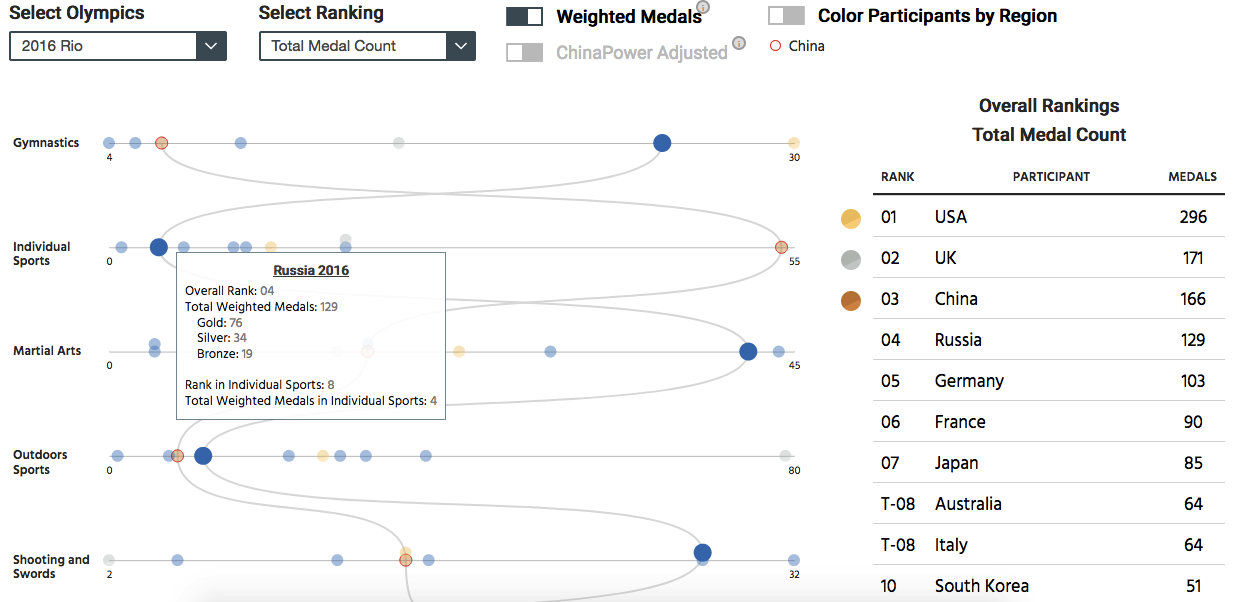
\includegraphics[width=0.95\linewidth]{static/pics/3-7} 

}

\caption{Ranking of countries by weighted medals}\label{fig:figure10}
\end{figure}

To solve these problems, we decided to rank countries by ``medal points'' as well, but on an interactive choropleth world map.

\hypertarget{lit-ranking}{%
\subsection{Ranking Sports by Number of Athletes}\label{lit-ranking}}

Dutta (2018) in his Kaggle post visualized the top 10 sports that USA excel by putting 10 boxes vertically with sports winning the most gold medals on top. See Figure \ref{fig:figure11}.

\begin{figure}

{\centering 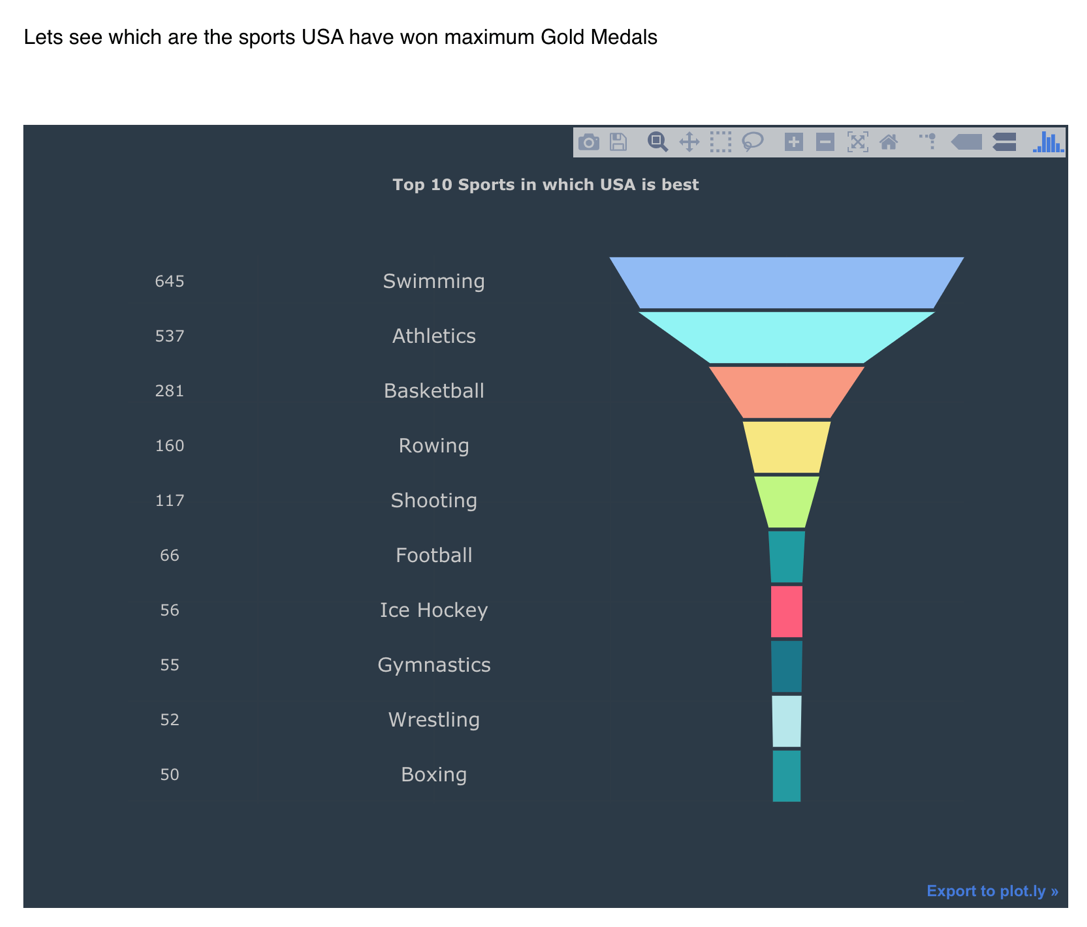
\includegraphics[width=0.9\linewidth]{static/pics/4-1} 

}

\caption{Ranking of sports by weighted medals}\label{fig:figure11}
\end{figure}

This visualization is transparent and clear but the problem is that it is limited to only about 10 items, which is not enough for us to visualize all the sports in the Summer Olympics. Instead, we decided to try a bar chart and word cloud for our visualizations.

\hypertarget{plans}{%
\section{Plans}\label{plans}}

In the following, we'll detail our plans for making visualizations.

\hypertarget{plans-female}{%
\subsection{Female Participation}\label{plans-female}}

As discussed above, we will use a line graph, stacked bar chart, and area chart to show the overall trend of female participation in the Summer Olympics. For female participation in each individual continent, we will use KDE in a small multiple.

In a line graph, the x-axis will be time and the y-axis the percentage against the total number of participants. We will show both female and male athletes. See Figure \ref{fig:figure12}.

For stacked bar charts, the x-axis will be time and y-axis percentage against the total number of athletes. Two segments in each bar will represent male and female respectively, and the two will sum up to 100\% for every year presented. This will make the comparison between male and female participation very clear. See Figure \ref{fig:figure13}.

\begin{figure}

{\centering 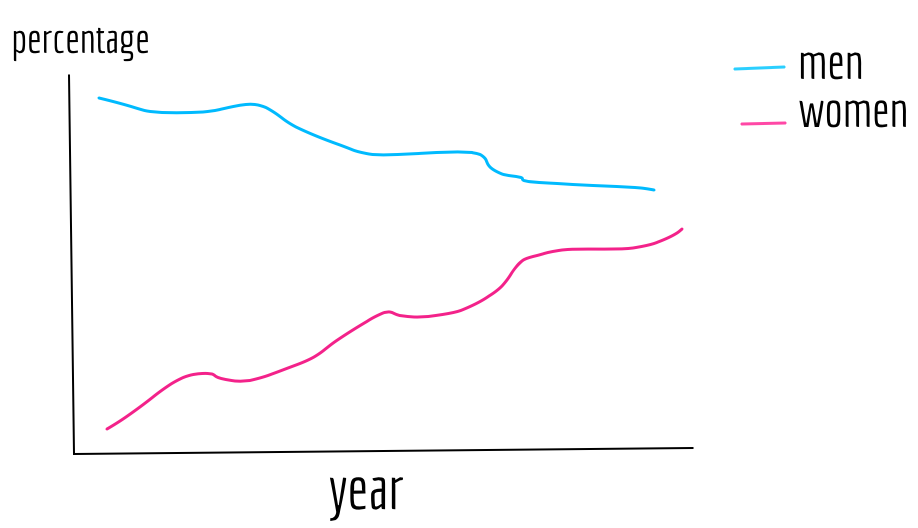
\includegraphics[width=0.85\linewidth]{static/pics/1} 

}

\caption{Line graph for female participation}\label{fig:figure12}
\end{figure}

\begin{figure}

{\centering 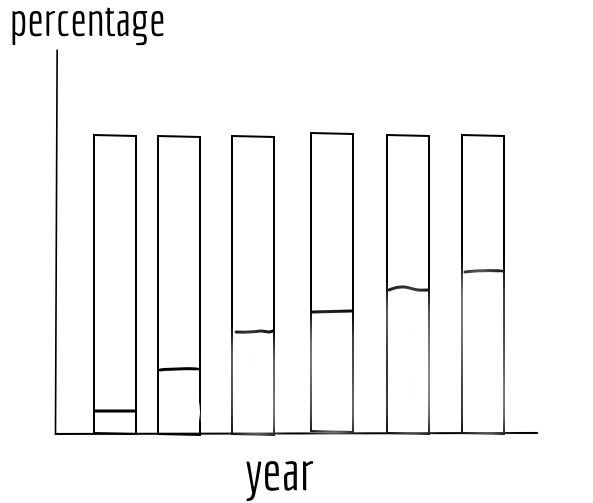
\includegraphics[width=0.75\linewidth]{static/pics/2} 

}

\caption{Stacked bar chart for female participation}\label{fig:figure13}
\end{figure}

In order to also show the changes in the total number of athletes, beside the changes in percentages, we will use a stacked area chart. The x-axis will be again time, and the y-axis will be the total number of athletes for each Olympic Games. See Figure \ref{fig:figure14}.

For female participation in each individual continent over the years, we will line graphs in a small multiple. The x-axis will be time and the y-axis will be the percentage of female athletes against the total number of athletes. To make comparisons between continents and with the global average clearer, for each plot in the small multiple, we will put the line graph of other continents in the background, and we will also plot the global average as the benchmark. See Figure \ref{fig:figure15}.

\begin{figure}

{\centering 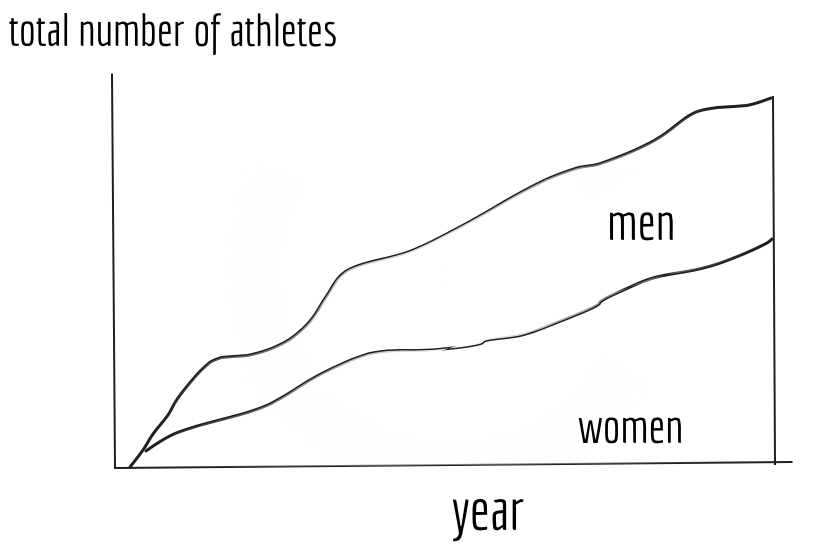
\includegraphics[width=0.75\linewidth]{static/pics/3} 

}

\caption{Staked area chart for female participation}\label{fig:figure14}
\end{figure}

\begin{figure}

{\centering 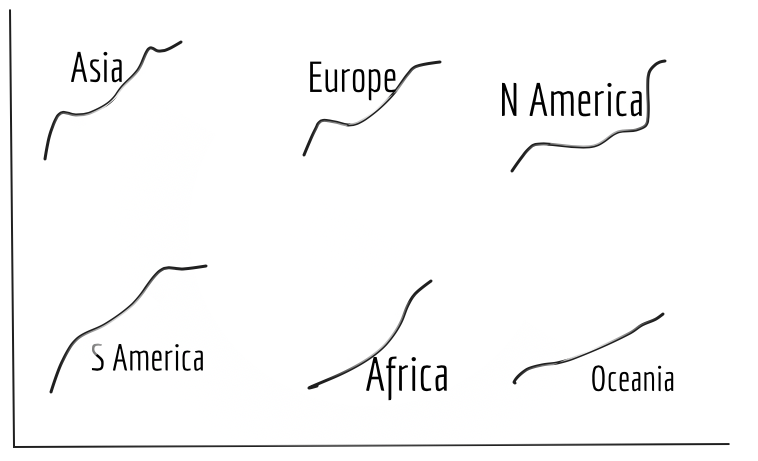
\includegraphics[width=0.75\linewidth]{static/pics/4} 

}

\caption{Line graph in small multiple for female participation}\label{fig:figure15}
\end{figure}

\hypertarget{plans-homefield}{%
\subsection{Home-field Advantage}\label{plans-homefield}}

To examine whether there exists a home-field advantage at the Olympics, we will first use a scatter plot with jitter. The x-axis will be countries that have ever been a host, and the y-axis will be the percentage against the total number of medals a country earned. Each dot represents an Olympic Games the country has participated in. Black dots denote data for a ``non-host'' year and orange dots denote data for host year. See Figure \ref{fig:figure16}.

To better show the density distribution of medal gains, we will employ kernel density estimation in a small multiple. The x-axis will be the percentage against the total number of medals at a Games and the y-axis will be density. We will use an arrow to denote the density of a year when the country was a host. See Figure \ref{fig:figure17}.

Arrows located at points with high densities, would be signs of the existence of home-field advantage at the Olympics.

\begin{figure}

{\centering 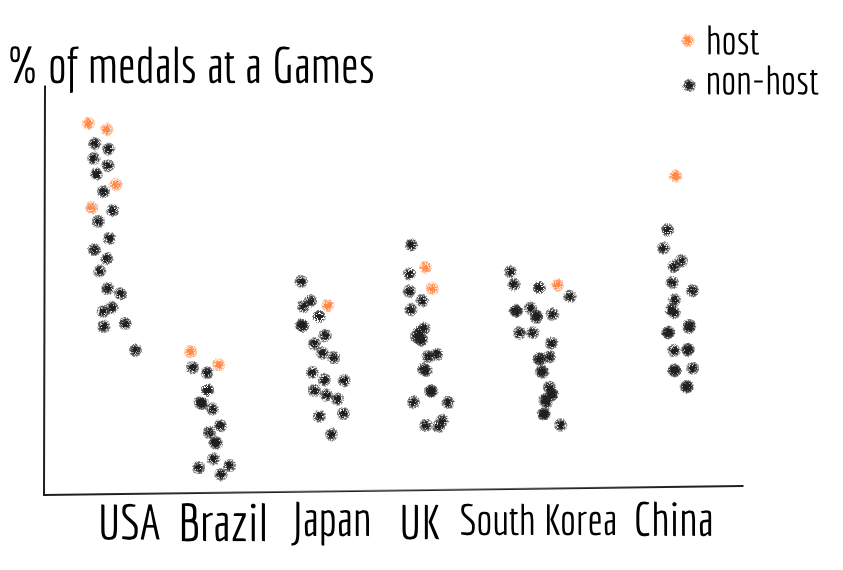
\includegraphics[width=0.8\linewidth]{static/pics/5} 

}

\caption{Scatter plot with jittering for home-field advantage}\label{fig:figure16}
\end{figure}

\begin{figure}

{\centering 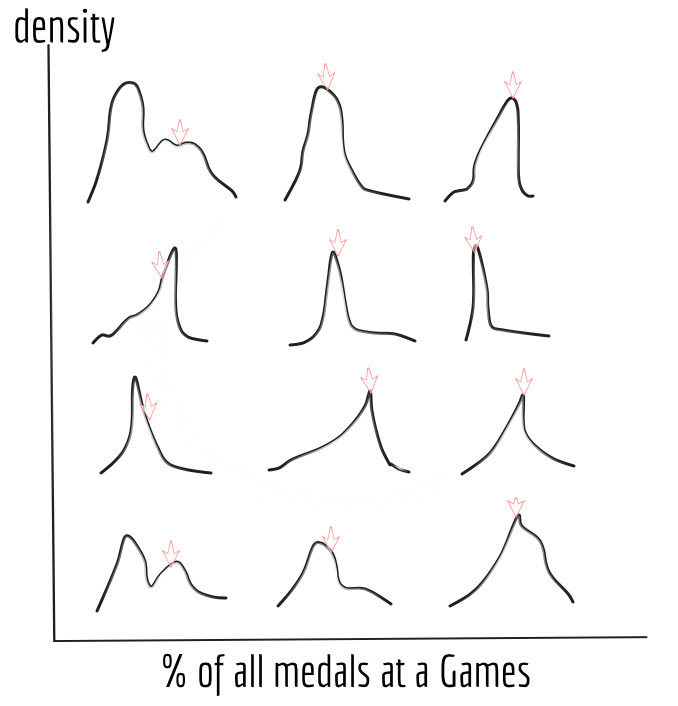
\includegraphics[width=0.75\linewidth]{static/pics/6} 

}

\caption{KDE for home-field advantage}\label{fig:figure17}
\end{figure}

\hypertarget{plans-medal-efficiency}{%
\subsection{Medal Efficiency}\label{plans-medal-efficiency}}

The index of ``medal efficiency'' will be calculated as medal points per athlete participating. We will use an interactive choropleth world map to show each participating country and region's score. See Figure \ref{fig:figure18}.

\begin{figure}

{\centering 
\includegraphics[width=0.95\linewidth]{static/pics/9} 

}

\caption{Choropleth map for medal efficiency}\label{fig:figure18}
\end{figure}

\hypertarget{plans-ranking}{%
\subsection{Ranking Sports}\label{plans-ranking}}

First, we will use a bar chart where the x-axis will be the different sports and the y-axis the corresponding number of athletes. See Figure \ref{fig:figure19}.

Second, we will show this ranking using a word cloud in which larger font size denotes a higher number of participants. This graph will be clearer and more direct because viewers can intuitively get a sense of the relative size of participation of a sport. See Figure \ref{fig:figure20}.

\begin{figure}

{\centering 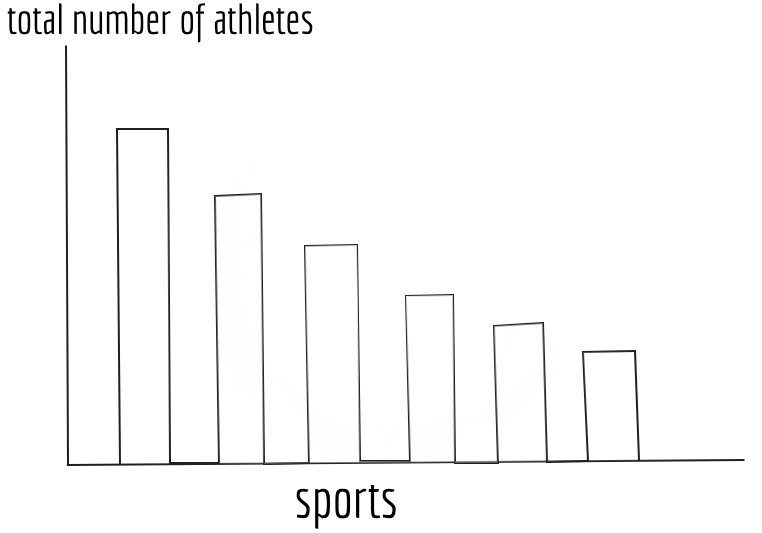
\includegraphics[width=0.85\linewidth]{static/pics/7} 

}

\caption{Bar chart for sports ranking}\label{fig:figure19}
\end{figure}

\begin{figure}

{\centering 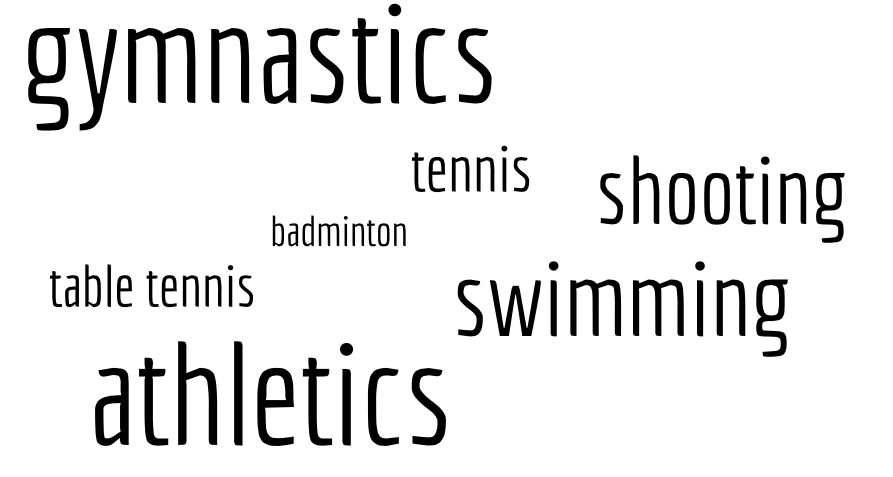
\includegraphics[width=0.85\linewidth]{static/pics/8} 

}

\caption{Word cloud for sports ranking}\label{fig:figure20}
\end{figure}

\hypertarget{plots}{%
\section{Plots}\label{plots}}

In the following, we'll show the final plots based on our plans.

\hypertarget{plots-female-time}{%
\subsection{Female Participation over Time}\label{plots-female-time}}

As planned above, we started with a simple line graph displaying both male and female athletes' percentage against all athletes. The strength of this method is that it is simple and clear. It shows that the female percentage has been steadily growing in the past century at the Olympics. The drawback is that it does not generate a stark contrast between male and female as a stacked bar chart can do. See Figure \ref{fig:figure21}.

\begin{figure}

{\centering 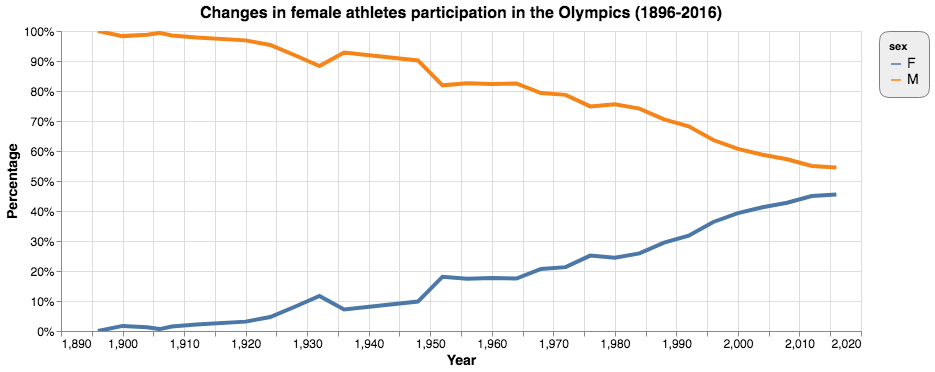
\includegraphics[width=1\linewidth]{static/pics/g-1-1} 

}

\caption{Line graph for changes in female participation}\label{fig:figure21}
\end{figure}

We then used stacked bar graphs. We first tried stacking the bar horizontally with percentage on the x-axis and time on y-axis. See Figure \ref{fig:figure22}.

\begin{figure}

{\centering 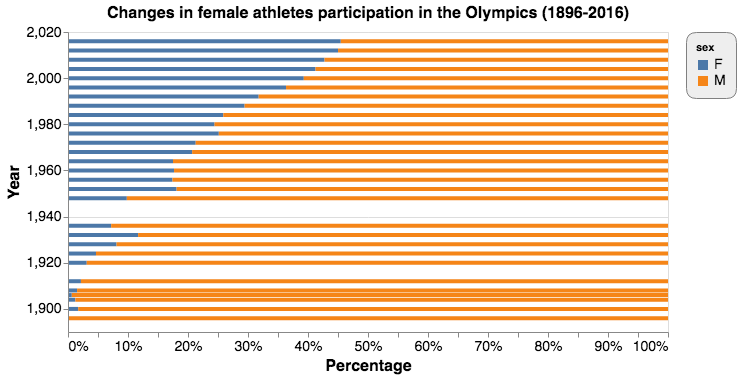
\includegraphics[width=1\linewidth]{static/pics/g-1-2} 

}

\caption{Horizontal stacked bar chart for changes in female participation}\label{fig:figure22}
\end{figure}

It was not as beautiful as we wanted, so we tried to put it upright and replace the axis labels. To highlight the trend, we set the male section grey and the female part bright blue. We also drew a red line at the intersection of the two parts. This time, female participation was obviously highlighted and the trend shown very clearly. See Figure \ref{fig:figure23}.

\begin{figure}

{\centering 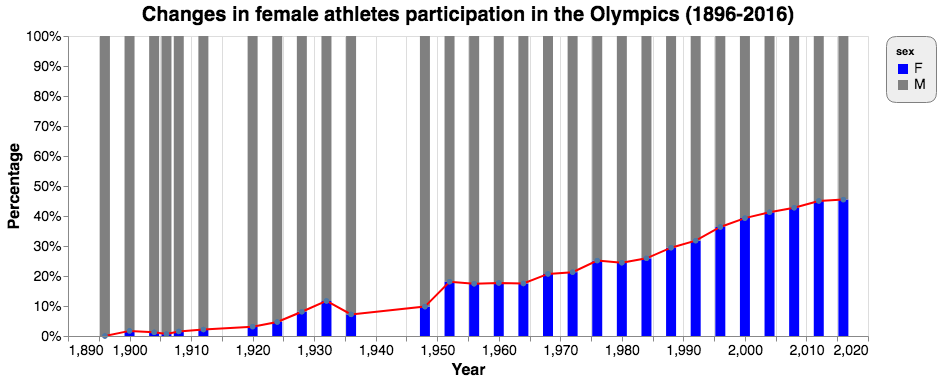
\includegraphics[width=1\linewidth]{static/pics/g-1-3} 

}

\caption{Vertical stacked bar chart for changes in female participation}\label{fig:figure23}
\end{figure}

However, as discussed above, stacked bar charts can only show the changes in percentages, not those in the actual number of participants. To also visualize how the total number of athletes participating in the Olympics changed over the century, we opted for a stacked area chart. See Figure \ref{fig:figure24}.

\begin{figure}

{\centering 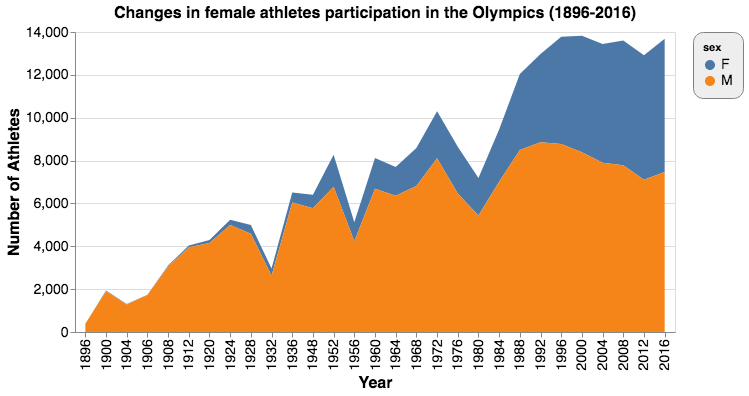
\includegraphics[width=1\linewidth]{static/pics/g-1-4_new} 

}

\caption{Stacked area chart for changes in female participation}\label{fig:figure24}
\end{figure}

The x-axis denotes time and the y-axis number of athletes. Areas are made up of male and female participants. The two added up to the total number of athletes. This stacked area chart not only shows the changes in female participation, it also displays how the total number of athletes has been increasing over the years. The drawback is that area is not a much preferred visual encoding. As a result, the comparison of percentages of male and female is not very accurate. That said, we think its strengths outweigh its disadvantages.

\hypertarget{plots-female-continents}{%
\subsection{Female Participation Across Continents}\label{plots-female-continents}}

To visualize changes in female participation in each continent, we first used a simple line graph where we put all the continent together. The x-axis is time, and the y-axis is female participation. The legend shows the colors associated with the continents. See Figure \ref{fig:figure25}.

\begin{figure}

{\centering 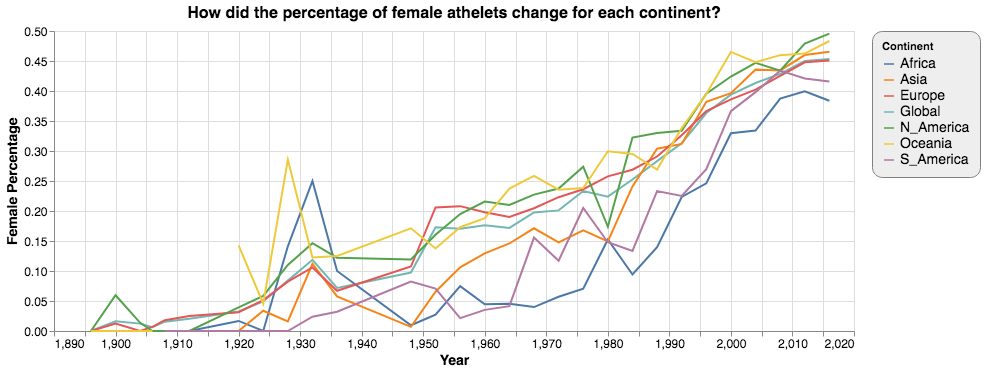
\includegraphics[width=1\linewidth]{static/pics/g-2-1_new} 

}

\caption{Line graph for female participation by continent}\label{fig:figure25}
\end{figure}

The graph was very messy. As there were six continents and one global average, we could not distinguish between the seven categories very easily. So we gave up this option.

Then we tried a small multiple in which each continent and the global average were shown in simple line graphs. This chart showed every continent clearly but it was not very easy to make a comparison. See Figure \ref{fig:figure26}.

\begin{figure}

{\centering 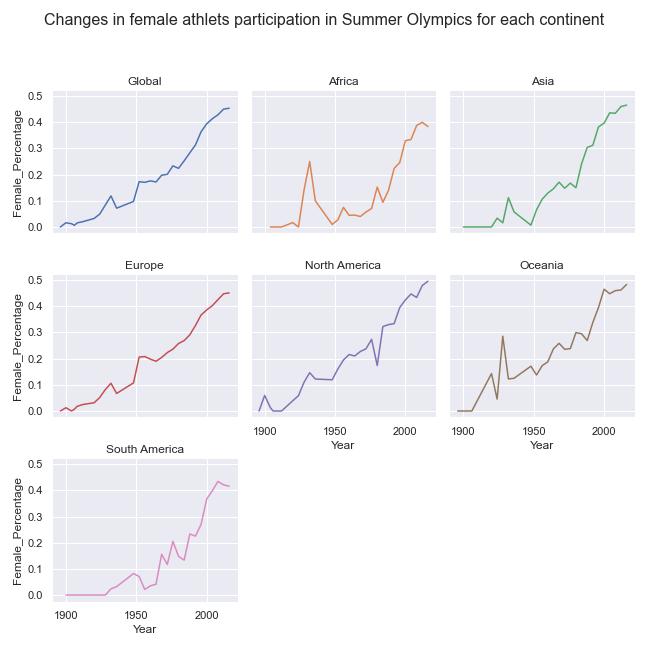
\includegraphics[width=1\linewidth]{static/pics/g-2-2} 

}

\caption{Line graph in small multiple for female participation by continent}\label{fig:figure26}
\end{figure}

To make comparisons clearer, we decided to use an area chart. We stacked each area chart each representing a continent along a vertical line. However, comparisons were still difficult. Most importantly, in terms of using color as the visual encoding, this graph has too many categories. Besides, it has red and green at the same time, and therefore is not accessible to colorblind populations. See Figure \ref{fig:figure27}.

\begin{figure}

{\centering 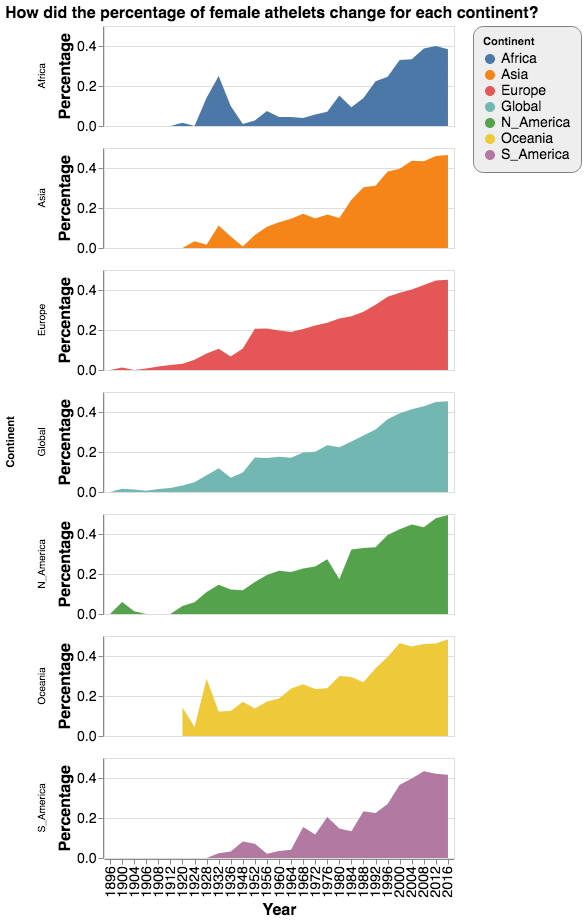
\includegraphics[width=0.8\linewidth]{static/pics/g-2-4_new} 

}

\caption{Stacked bar chart for female participation by continent}\label{fig:figure27}
\end{figure}

We then went back to the small multiple. Since we cared about the comparison between each continent, we decided to plot every continent and the global average in each of the six graphs. We highlighted only one continent in each graph, and set all other continents grey in the background. It worked much better than out earlier attempts, but one drawback is that it did not allow comparison with the global average. See Figure \ref{fig:figure28}.

\begin{figure}

{\centering 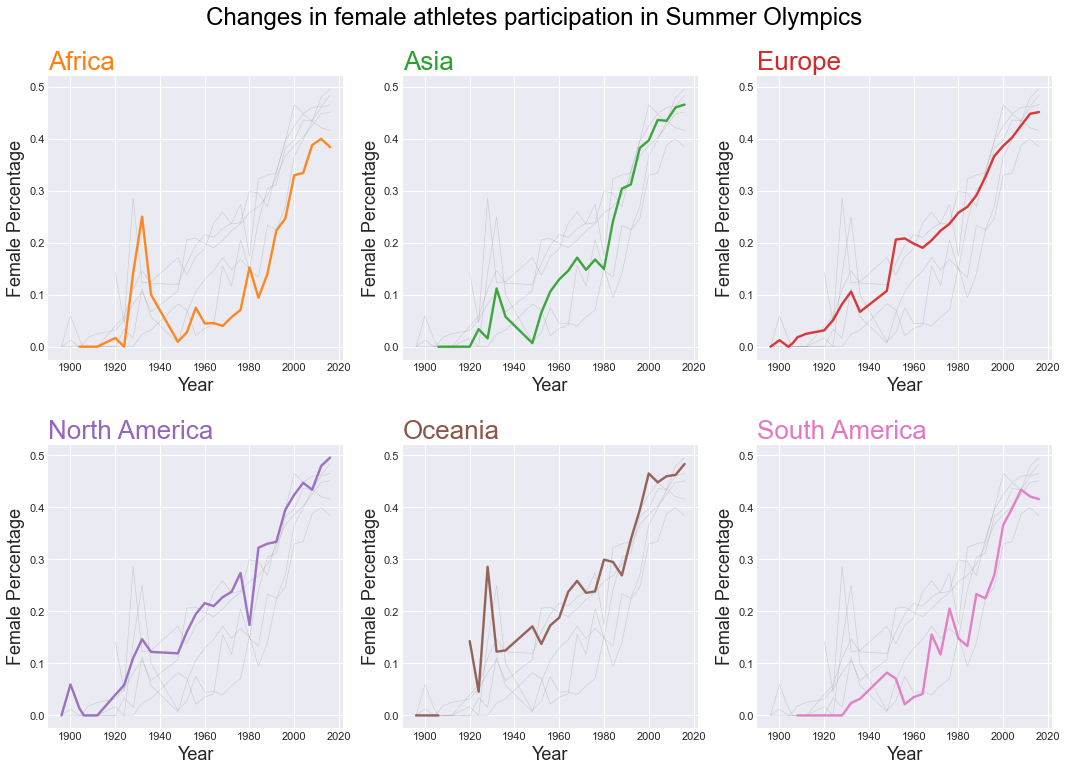
\includegraphics[width=1\linewidth]{static/vis/g-2-5} 

}

\caption{Line graph in small multiple for female participation by continent against all other groups}\label{fig:figure28}
\end{figure}

Finally, we decided to highlight the global average with a black line. This time, comparisons both between continents and with the global average were clear. See Figure \ref{fig:figure29}.

\begin{figure}

{\centering 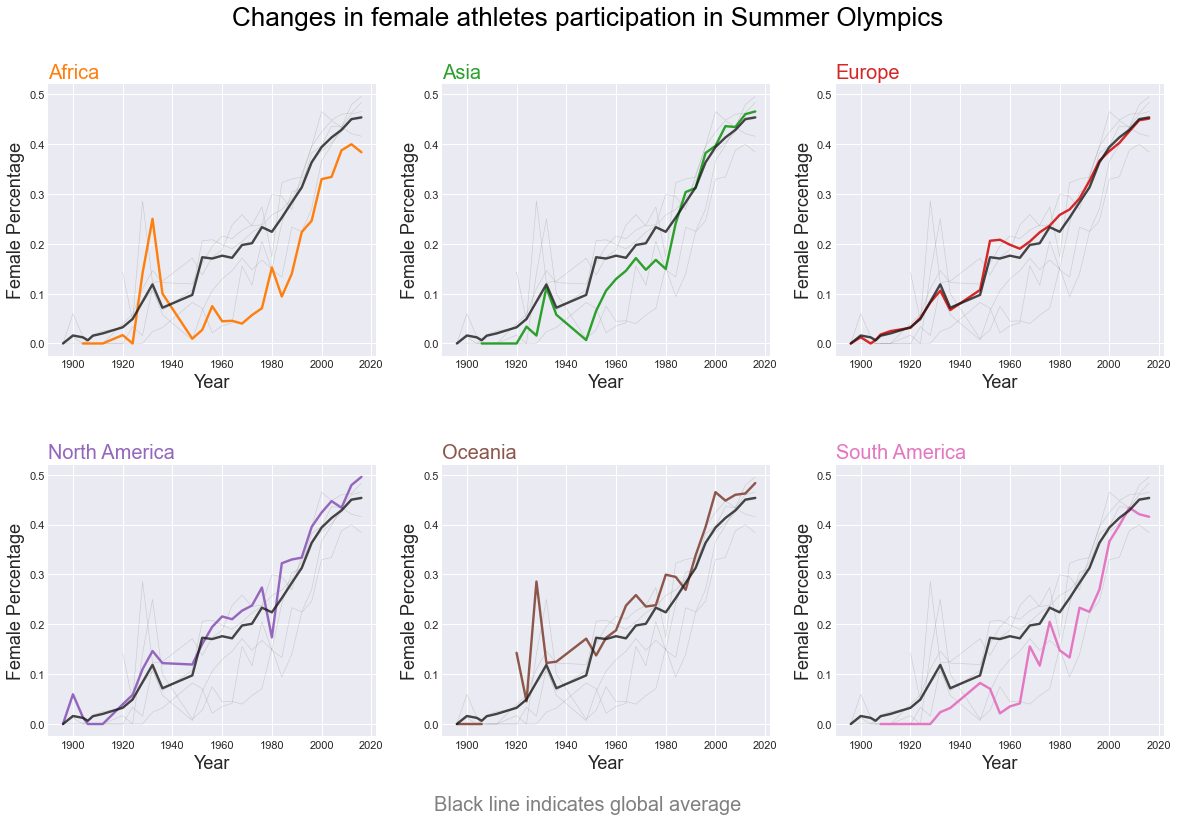
\includegraphics[width=1\linewidth]{static/vis/g-2-6} 

}

\caption{Line graph in small multiple for female participation by continent against global statistics}\label{fig:figure29}
\end{figure}

\hypertarget{plots-homefield}{%
\subsection{Home-field Advantage}\label{plots-homefield}}

As discussed above, we first tried scatter plot with jitter. The x-axis is the countries that have ever hosted the Olympics and the y-axis denotes the percentage of medals earned by a country against the total number of medals in that year. Blue dots represent data when the country was not the host and the orange ones for when it was the host. See Figure \ref{fig:figure30}.

\begin{figure}

{\centering 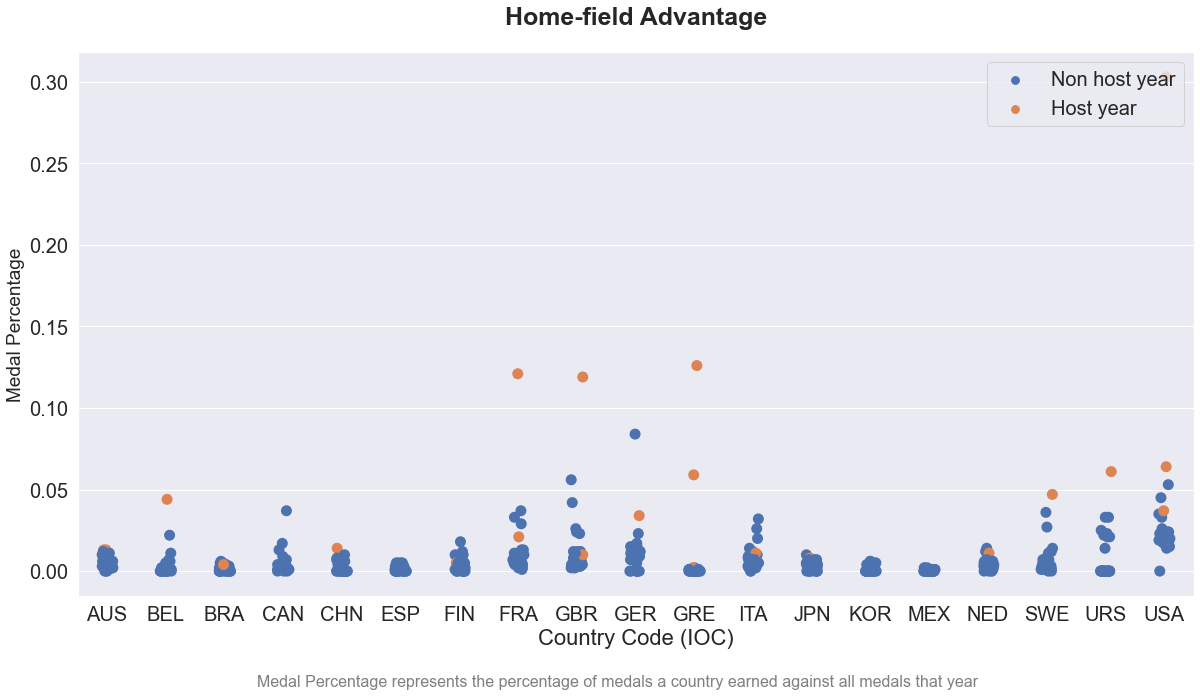
\includegraphics[width=1\linewidth]{static/vis/g-2-7} 

}

\caption{Scatter plot with jittering for home-field advantage}\label{fig:figure30}
\end{figure}

The blue dots were too packed. We later tried beeswarm plot coupled with box plot. Dots were shown much more clearly but one drawback is that we could not see the density distribution of all the dots very well. Density distribution was important in this case because it would allow an easier comparison between the medal percentage when a country was a host and that when it was not. See Figure \ref{fig:figure31}.

\begin{figure}

{\centering 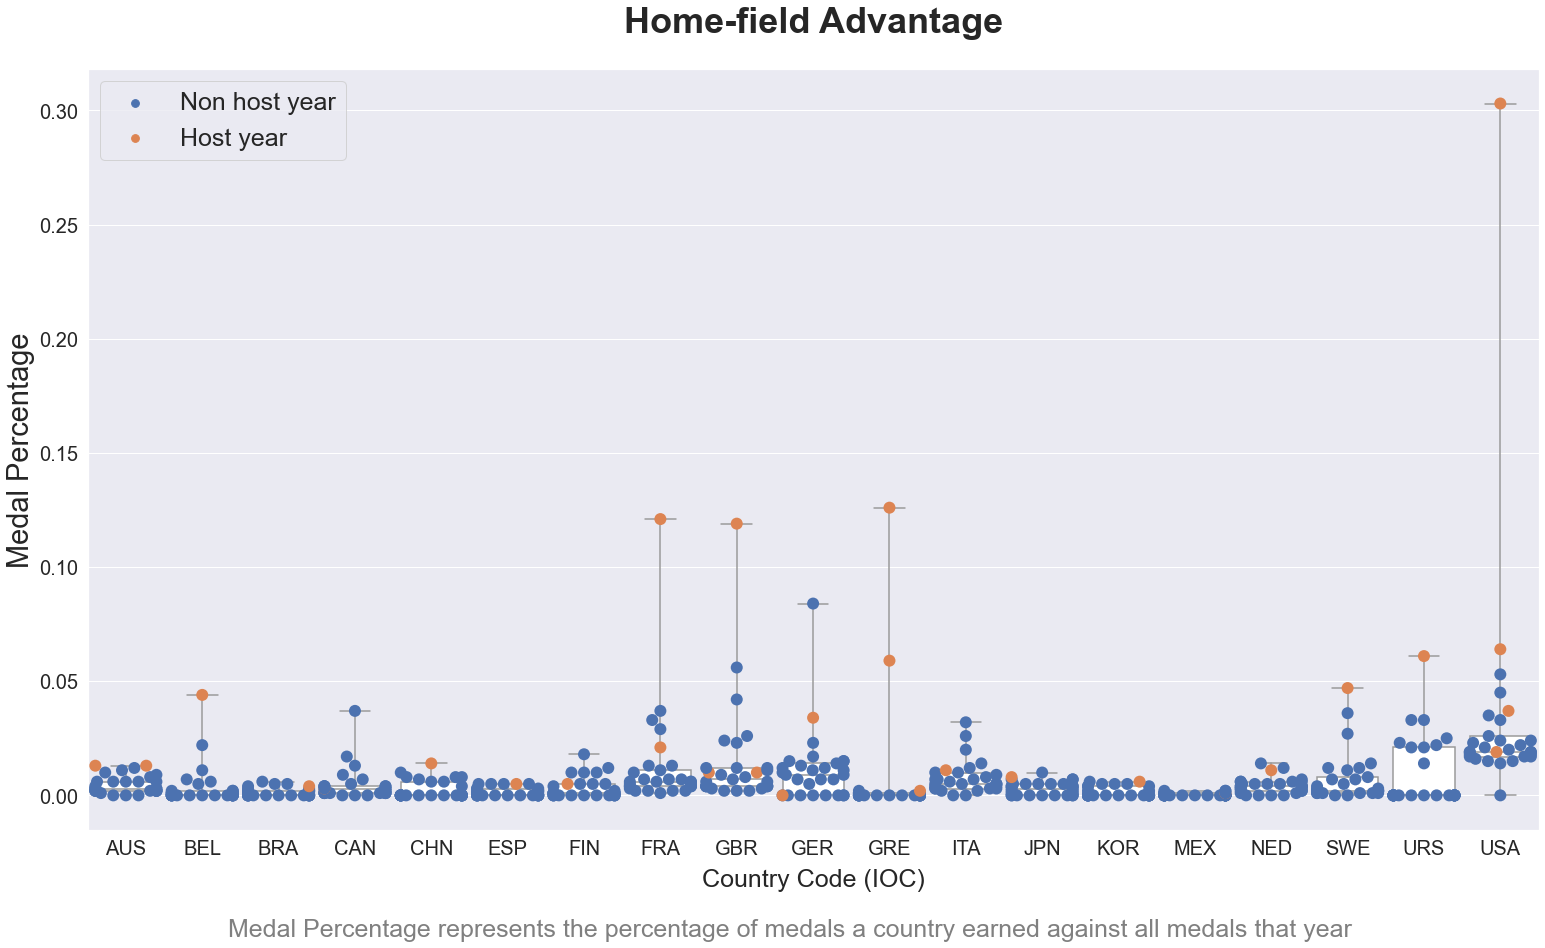
\includegraphics[width=1\linewidth]{static/vis/g-2-8} 

}

\caption{Beeswarm plot for home-field advantage}\label{fig:figure31}
\end{figure}

To show density distribution of medal percentages, we used kernel density estimation in a small multiple. The x-axis is the medal percentage and the y-axis is the probability density. We used a red arrow to denote when the country was an Olympics host. An arrow located at the tail would indicate the existence of home-field advantage. See Figure \ref{fig:figure32}.

\begin{figure}

{\centering 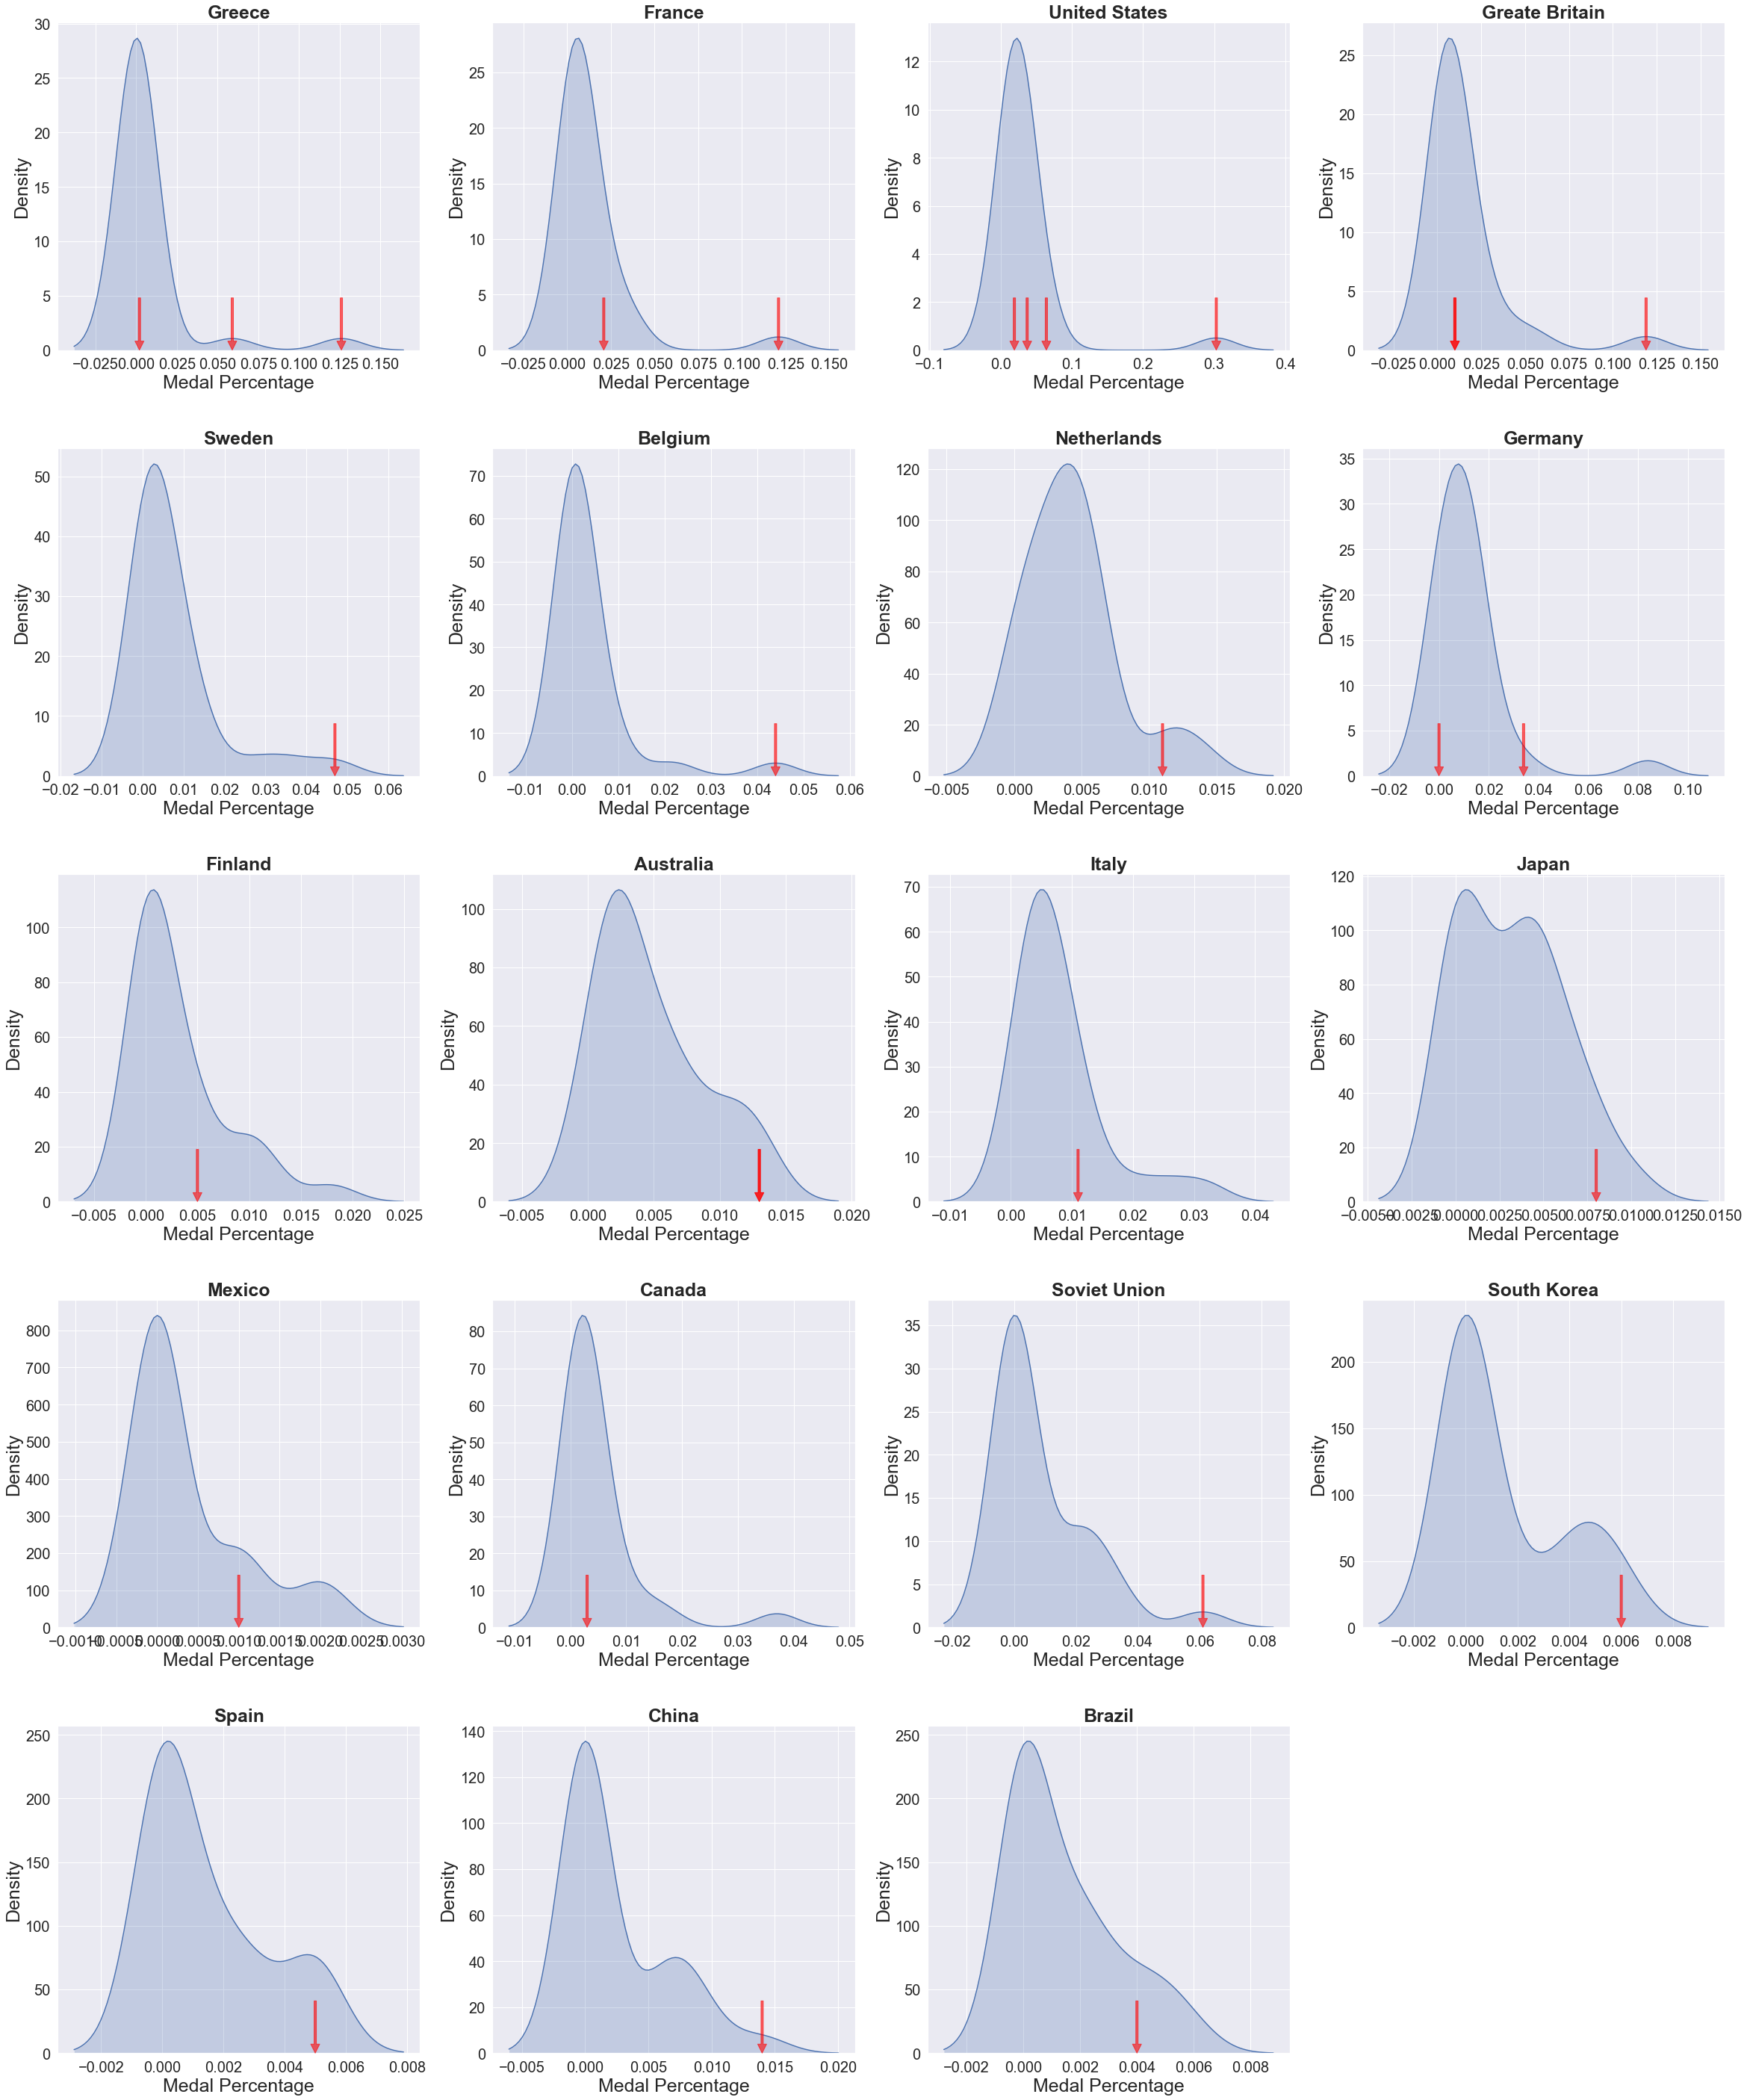
\includegraphics[width=1\linewidth]{static/pics/g-2-9} 

}

\caption{KDE in small multiple for home-field advantage}\label{fig:figure32}
\end{figure}

\hypertarget{plots-medal-efficiency}{%
\subsection{Medal Efficiency}\label{plots-medal-efficiency}}

As planned, first of all, we did data manipulation before plotting. Golds were given 4 points, Silver 2, and Bronze 1. Attendance without any medals was assigned to 0 point. A country's ``medal efficiency'' was calculated as the quotient of total medal points and the total number of athletes participating over 120 years. Therefore, if a country/region has a medal efficiency of 0.5, it means that on average, each athlete of that country/region earned half a Bronze.

We then plotted a choropleth map using orthographic projection. We applied Viridis color map where darker shades denote higher medal efficiency. To ensure interactivity, we made this map with the Plotly package. See Figure \ref{fig:figure33}.

\begin{figure}

{\centering 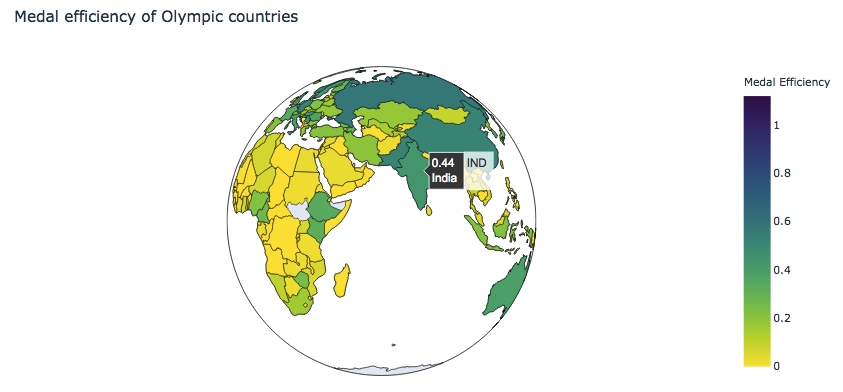
\includegraphics[width=1\linewidth]{static/pics/g-3-1} 

}

\caption{Interactive choropleth for medal efficiency}\label{fig:figure33}
\end{figure}

We found this index both more accurate and intuitive. The reasons why it is more accurate have been outlined above. We believe that it is also more intuitive because, for example, for countries that still exist today, the highest medal efficiency is 0.91 for the United States of America. The fact that the highest is close to one makes it easier to compare between countries.

\hypertarget{plots-ranking}{%
\subsection{Ranking Sports}\label{plots-ranking}}

To rank sports according to the number of athletes, we first plotted a bar chart, each bar representing a category. As can be seen below, since there were too many categories, the names of sports overlapped to a degree that most of them were indistinguishable. Since there are around thirty sports, using colors is not an ideal option.

We then thought about the word cloud. In word clouds, the size of words is associated with the frequencies. This would make our ranking clearer. We did this visualization with the \texttt{wordcloud} package. See Figure \ref{fig:figure34}.

\begin{figure}

{\centering 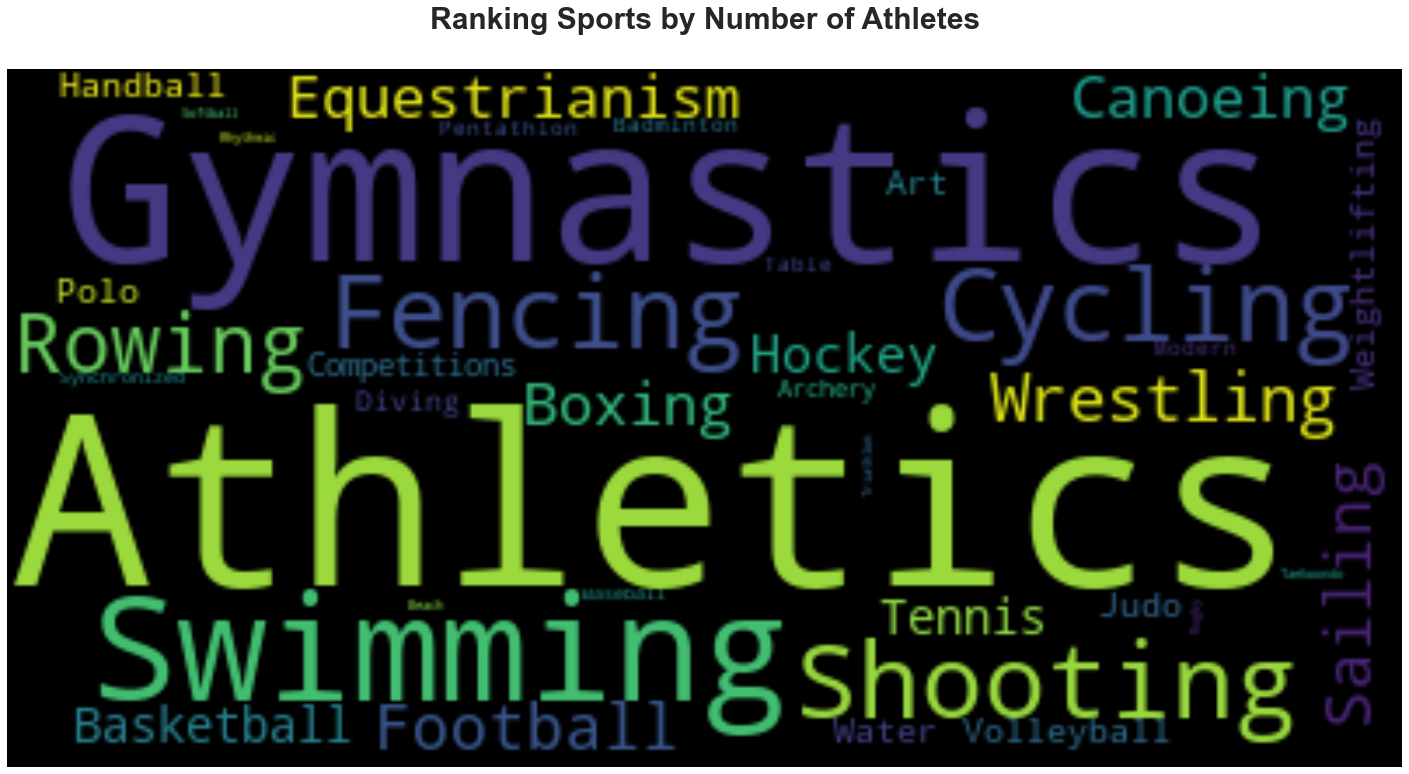
\includegraphics[width=1\linewidth]{static/pics/g-4-2} 

}

\caption{Word cloud of sports ranking by number of participants in all past Summer Olympics}\label{fig:figure34}
\end{figure}

\hypertarget{conclusion}{%
\section{Conclusion}\label{conclusion}}

We'll conclude by recapping our major questions and findings. We'll also offer advice on future studies.

\hypertarget{conclusion-rq-recap}{%
\subsection{Research Question Recap}\label{conclusion-rq-recap}}

This paper answered four major questions:

\begin{itemize}
\tightlist
\item
  How does female participation at the Olympics, both overall and in each continent, change over time?
\item
  Is there a home-field advantage at the Olympics?
\item
  What is the medal efficiency for each country and region?
\item
  Which sports have the highest number of participating athletes at the Olympics?
\end{itemize}

\hypertarget{conclusion-findings}{%
\subsection{Major Findings}\label{conclusion-findings}}

Our visualizations demonstrated that:
- Both the total number of participating athletes and the percentage of female athletes in the Olympics has been increasing. Female participation started from 0\% in Athens 1896 to 45\% in Rio 2016.

\begin{itemize}
\item
  However, this growth in the rate of participation of women varies across continents. The rate in Africa has always been lower than the global average except for during the 1930s. The rate in Asia and South America had also been always lower than the global average but caught up during the 1980s and 2000s, respectively. The rate in Europe, North America and Oceania has always been the same as or higher than the global mean.
\item
  A country is more likely to have a higher degree of medal share when it hosts the Olympics. In other words, home-field advantage does seem to exist in the Olympics.
\item
  Among today's countries and regions, the United States of America has the highest medal efficiency, 0.91. This means that on average, every American athlete almost earned a Bronze medal in the past Olympic Games. Medal efficiency for Russia, China, Pakistan, India, Germany, and Australia is also very high. We also found that medal efficiency had a high correlation with countries' economic development.
\item
  Athletics, gymnastics, swimming, shooting and football are among the sports with the highest number of participating athletes. This might be because these sports have greater shares of total medals. It might also because there are many sub-categories within them.
\end{itemize}

\hypertarget{conclusion-reflections}{%
\subsection{Reflections \& Future Work}\label{conclusion-reflections}}

First, when visualizing changes in female participation, we found that stacked bar charts are effective in showing the comparisons between male and females. Stacked area charts do not provide very accurate percentage change, but it is good if we also want to show how the total number of athletes has been increasing. The seaborn FacetGrid function is useful for visualizing female participation by continent. Reference information set in grey in the background and highlighting the global average helps us make comparisons between continents and with the global average much clearer. Our next step is to do this graph with Altair so as to enable interactivity when we post it online.

In our study into the home-field advantage, we realized that even with jittering, scatter plot is not effective at showing a large number of data points. Beeswarm plot with box plot is good at displaying all the points without overlapping, but its representation of density distribution is not very intuitive and direct. KDE in a small multiple is a much better method for showing the distribution clearly. KDE in this case is especially useful for examining home-field advantage because it shows the level of probability that a country gets a certain share of medals.

Our introduction of ``medal efficiency'' contributes to the assessment of a country's efficiency at obtaining Olympic medals. The choropleth we used allows us to show all the countries and regions interactively. However, we acknowledged that it would have been better if it were a cartogram. This might be our next step.

Using word cloud is a very unique way to show the relative size of participation in various sports. The drawback is that some sports have two or more words in their names, and our processing of word clouds might not have been rendering their frequencies very accurately. That is why we see ``water'', ``art'' and ``competition'' in the word cloud. We will fix this problem in our next step.

We will publish it online as our portfolio later.

\hypertarget{references}{%
\section*{References}\label{references}}
\addcontentsline{toc}{section}{References}

Abrams, O. (2019, June 23). Why Female Athletes Earn Less Than Men Across Most Sports. Retrieved from \url{https://www.forbes.com/sites/oliviaabrams/2019/06/23/why-female-athletes-earn-less-than-men-across-most-sports/\#646f8eeb40fb}.

Baker, C. N., Seymour, E., \&Zimbalist, A. (2019, April 18). Less Money, Less Media: How Female Athletes are Undervalued. Retrieved from \url{https://msmagazine.com/2019/04/18/less-money-less-media-how-female-athletes-are-undervalued/}.

Bian, X. (2005). Predicting Olympic medal counts: The effects of economic development on Olympic performance. \emph{The park place economist, 13}(1), 37-44.

Beutler, I. (2008). Sport serving development and peace: Achieving the goals of the United Nations through sport. \emph{Sport in society, 11}(4), 359-369.

Bernard, A. B., \& Busse, M. R. (2004). Who wins the Olympic Games: Economic resources and medal totals. \emph{Review of economics and statistics, 86}(1), 413-417.

COC. (2014, March 27). 10th-15th Olympic Games: 1936-1952. Retrieved from \url{http://en.olympic.cn/games/summer/2004-03-27/121663.html}.

Cooky, C., Messner, M. A., \& Musto, M. (2015). ``It's dude time!'' A quarter century of excluding women's sports in televised news and highlight shows. \emph{Communication \& Sport, 3}(3), 261-287.

Cottrell, M. P., \& Nelson, T. (2011). Not just the Games? Power, protest and politics at the Olympics. \emph{European Journal of International Relations, 17}(4), 729-753.

Darnell, S. C. (2012). Olympism in action, Olympic hosting and the politics of `sport for development and peace': Investigating the development discourses of Rio 2016. \emph{Sport in Society, 15}(6), 869-887.

Dutta, D. (2018). Analysing the Olympics (for last 120 yrs.). Retrieved from \url{https://www.kaggle.com/duttadebadri/analysing-the-olympics-for-last-120-yrs}.

Farmer, I. (2017, December 18). Why are female athletes paid less than male athletes? Retrieved from \url{https://news.jrn.msu.edu/2017/12/why-are-female-athletes-paid-less-than-male-athletes/}.

Forbes (2019). World's Highest Paid Athletes. Retrieved from \url{https://www.forbes.com/athletes/list//\#tab:overall}.

Ghildiyal, R. (2015). Role of sports in the development of an individual and role of psychology in sports. Retrieved from \url{https://www.ncbi.nlm.nih.gov/pmc/articles/PMC4381313/}.

Giulianotti, R. (2015). The Beijing 2008 Olympics: Examining the interrelations of China, globalization, and soft power. \emph{European Review, 23}(2), 286-296.

Goldblatt, D. (2016, August 4). Nobody wants to host the Olympic Games anymore. Can you blame them? Retrieved from \url{https://qz.com/748894/nobody-wants-to-host-the-olympic-games-anymore-can-you-blame-them/}.

Good, A. (2015, June 5). When it comes to women in sports, TV news tunes out. Retrieved from \url{https://news.usc.edu/82382/when-it-comes-to-women-in-sports-tv-news-tunes-out/}.

Grix, J. (2013). Sport politics and the Olympics. \emph{Political studies review, 11}(1), 15-25.

Center for Strategic International Studies (n.d.). How dominant is China at the Olympic Games? Retrieved from \url{https://chinapower.csis.org/dominant-china-olympic-games/}.

International Table Tennis Federation. (2018). Tyko 2020 Qualification System Table Tennis (Eng). Retrieved from \url{https://www.ittf.com/wp-content/uploads/2018/05/2018-05-14-Tokyo-2020-Qualification-system-Table-Tennis-eng.pdf}

Johnson, I. (2008, August 13). Who's on First in Medals Race? Retrieved from \url{https://www.wsj.com/articles/SB121856271893833843?ns=prod/accounts-wsj}.

Klein, J. Z. (2008, August 23). The Medal Rankings: Which Country Leads the Olympics? {[}FINAL UPDATE{]}. Retrieved from \url{https://beijing2008.blogs.nytimes.com/2008/08/23/the-medal-rankings-which-country-leads-the-olympics/}.

Ludacer, R. (2018, February 6). No one wants to host the Olympics anymore - will they go away? Retrieved from \url{https://www.businessinsider.com/future-olympics-no-country-wants-to-host-games-2018-2}.

MacAloon, J. (1995). Politics and the Olympics: some new dimensions. Received from \url{https://www.recercat.cat/bitstream/handle/2072/10632/WP053_eng.pdf?sequence=1}

MacKenzie, M. (2019, July 16). Female Athletes Receive Only 4\% of Sports Media Coverage-Adidas Wants to Change That. Retrieved from \url{https://www.glamour.com/story/female-athletes-receive-only-4-of-sports-media-coverage-adidas-wants-to-change-that}.

Malfas, M., Theodoraki, E., \& Houlihan, B. (2004, September). Impacts of the Olympic Games as mega-events. In \emph{Proceedings of the Institution of Civil Engineers-Municipal Engineer\} (Vol. 157, No.~3, pp.~209-220}. Thomas Telford Ltd.

Mervosh, S., \& Caron, C. (2019, March 8). 8 Times Women in Sports Fought for Equality. Retrieved from \url{https://www.nytimes.com/2019/03/08/sports/women-sports-equality.html}.

Mower, J. (2012, January 1). London 2012: Olympic success is key to national pride. Retrieved from \url{https://www.bbc.com/news/world-16245075}.

Nunes, R.A. (2019). Women athletes in the Olympic Games. \emph{Journal of Human Sport and Exercise. 2019, 14}(3): 674-683. \url{doi:10.14198/jhse.2019.143.17}

Osada, M., Ojima, M., Kurachi, Y., Miura, K., \& Kawamoto, T. (2016). Economic impact of the Tokyo 2020 Olympic games. Bank of Japan Reports and Research Paper, Tokyo, January. Retrieved from \url{http://www.trustfu.com/Uploads/image/20180827/20180827212024_95674.pdf}

Rathke, A., \& Woitek, U. (2007). Economics and Olympics: An efficiency analysis. Available at SSRN 967629.

Sandercock, G., Beedie, C., \& Mann, S. (2016). Is Olympic inspiration associated with fitness and physical activity in English schoolchildren? A repeated cross-sectional comparison before and 18 months after London 2012. \emph{British Medical Journal Open, 6}(11).

Soós, I., Martínez, J. C. F., \& Szabo, A. (2017). Before the Rio Games: A retrospective evaluation of the effects of the population size, GDP and national temperature on winning medals at the 2012 London Olympic Games. \emph{Journal of Human Sport and Exercise, 12}(1), 246-250.

Wikipedia (n.d.). Retrieved from \url{https://en.wikipedia.org/wiki/Table_tennis_at_the_2020_Summer_Olympics_–_Qualification}.

Warburton, D. E., Nicol, C. W., \& Bredin, S. S. (2006). Health benefits of physical activity: the evidence. \emph{Cmaj, 174}(6), 801-809.

World Bank (2018). Population 2018. Retrieved from \url{https://databank.worldbank.org/data/download/POP.pdf}

\end{document}
